\documentclass{article}
\usepackage[utf8]{inputenc}
\usepackage{todonotes}
\usepackage[colorlinks=true, allcolors=blue]{hyperref}


\title{rapport}
\author{jjycavailles }
\date{May 2019}

%\usepackage{natbib}

%\usepackage[authoryear]{natbib}
%\usepackage{biblatex}
\usepackage[round]{natbib}
%\usepackage{natbib}

%\bibliographystyle{plainnat}
%\usepackage[round]{natbib}

%\usepackage{cite}
%\setcitestyle{authoryear, open={((},close={))}

%\bibliography{references.bib}
%\bibliography{intro.bib}
%\addbibresource{intro.bib}
%\bibliographystyle{apalike}
%\usepackage[style=authoryear]{biblatex}
%\setcitestyle{authoryear,open={((},close={))}}

%\bibliographystyle{apalike}


\usepackage{graphicx}


%\usepackage{hyperref}
\usepackage[colorlinks=true, allcolors=blue]{hyperref}





\begin{document}

\begin{titlepage}

\begin{center}
  
\includegraphics[width = 25mm]{LogoInsa.png} \hfill
  
\includegraphics[width = 30mm]{logo_cnrs.jpg}
\end{center}

%\title{\textbf{Rapport de stage} \\ Ingenieur en mathematique \\ \textbf{ etude de la classification en regimes de temps et de leurs impacts pour des utilisations metiers.} }
%\author{Jerome Cavailles \\ $4^{ieme}$ annee, Genie mathematique et modelisation \\ INSA Toulouse}
%\date{28/06/2018 - 07/09/2018}




\vspace*{1cm}

\begin{center}
\rule{\linewidth}{0.7mm} \\
[0.4cm]
\textbf{ \Huge Internship report} \\
[0.2cm]
\large \emph{Engineer in mathematics} \\ 
[0.6cm]
\textbf{ \huge Destabilizing effects of controlling ecosystem behavior} \\
[0.4cm]
03/01/2019 - 08/30/2019 \\
[0.4cm]
\rule{\linewidth}{0.7mm}
\end{center}

\vspace*{0.5cm}

\begin{center}
\textbf{\Large{Jerome Cavailles}} \footnote{\url{jcavaill@etud.insa-toulouse.fr}} \\ [0.3cm] $5$ years, Mathematical engineering and modeling %\\ INSA Toulouse
\end{center}

%^{\text{ieme}}

%\maketitle

%\vspace*{2.5cm}
\vspace*{1.9cm}

\begin{flushleft}
Supervisor : Yuval Zelnik \footnote{\url{yuval.zelnik@sete.cnrs.fr}} \hfill
Tutor : Marie-Hélène Vignal \footnote{\url{marie-helene.vignal@math.univ-toulouse.fr}} \\  
Michel Loreau \footnote{\url{michel.loreau@sete.cnrs.fr}} \hfill
Charles Dossal \footnote{\url{dossal@insa-toulouse.fr}} \\
Laboratory : CNRS-Moulis \footnote{2, route du CNRS - 09200 Moulis, France, \url{http://www.cbtm-moulis.com}} \hfill 
University : INSA Toulouse \footnote{135, Avenue de Rangueil 31077 Toulouse Cedex 4, \url{http://www.insa-toulouse.fr}} \\
\hfill Paul Sabatier \footnote{118 route de Narbonne, 31062 Toulouse Cedex 9, \url{http://www.univ-tlse3.fr/}}
\end{flushleft}

%\paragraph{}
%\begin{tabbing}
%\hspace{2cm}\=\hspace{6cm}\=\hspace{2cm}\=\kill
%Supervisor \> Yuval Zelnik \footnote{\url{yuval.zelnik@sete.cnrs.fr}} \>
%Tutor \> Marie-Hélène Vignal \footnote{\url{marie-helene.vignal@math.univ-toulouse.fr}} \\  
%\> Michel Loreau \footnote{\url{michel.loreau@sete.cnrs.fr}} 
%\> \> Charles Dossal \footnote{\url{dossal@insa-toulouse.fr}} \\
%Laboratory \> CNRS-Moulis \footnote{2, route du CNRS - 09200 Moulis, France, \url{http://www.cbtm-moulis.com}} \> University \> INSA Toulouse\footnote{135, Avenue de Rangueil 31077 Toulouse Cedex 4} \\
%\>\>\> Paul Sabatier \footnote{118 route de Narbonne, 31062 TOULOUSE CEDEX 9 \url{http://www.univ-tlse3.fr/}}
%\end{tabbing}

\end{titlepage}



\newpage
%\addto\captionsfrench{\def\contentsname{}} % pour supprimer le "table des matieres en haut"

\paragraph{}
%\section*{Contents}

\addcontentsline{toc}{section}{Contents}

\tableofcontents



\newpage
%\section*{Liste des figures, des tables et des algorithmes}
%\addcontentsline{toc}{section}{Liste des figures, des tables et des algorithmes}
%\paragraph{}
\addcontentsline{toc}{section}{List of figures}
\listoffigures

\newpage
\addcontentsline{toc}{section}{Abbreviations /Glossary}
\todo{use nomenclature packages}
\section*{Abbreviations / Glossary}
%\listoffigures





\newpage
\section*{Acknowledgment}
\addcontentsline{toc}{section}{Acknowledgment}



\newpage
%\todo{Choice of this internship ?}
\section*{Introduction}
\addcontentsline{toc}{section}{Introduction}

\subsection*{Station presentation}
\addcontentsline{toc}{subsection}{Station presentation (1-2 pages)}

\paragraph{}
The CNRS\footnote{\url{http://www.cnrs.fr/en/cnrs}}, the Scientific Research National Center (in french, Centre National de la Recherche Scientifique) was created on the 19th of October, 1939. It is a world renowned research institution, ranked second by  nature index \footnote{\url{https://www.natureindex.com/institution-outputs/generate/All/global/All/n_article}}. It has approximately 33,000 researchers working in 1,144 laboratories throughout France and abroad, with a budget around 3 billion euros. 

The CNRS is currently headed by Antoine Petit (President and CEO), and its laboratories are organised in two types: proper units (UPRs) and mixed units (UMRs), the latter being managed in association with other French institutions (higher education establishment or another research institution). In addition, there are 36 international Joint Units (UMI) of collaborations around the world. The CNRS conducts research in all disciplines of basic research (Ecology and environment, Humanities and social sciences, Engineering and systems, Mathematics, Physics, Information sciences, etc. , ).


\paragraph{}
One of these mixed research units (UMR 5321) is the Station for Theoretical and Experimental Ecology\footnote{\url{https://sete-moulis-cnrs.fr}} (SETE), located in Moulis\footnote{\url{http://www.communes.com/midi-pyrenees/ariege/moulis_09200/}} (Ariege, France). It was originally founded in 1948 by professors Jeannel and Vandel, due to its vicinity to many caves, with the aim of the station to use the underground cave systems in order to study the formation and physical properties of karstic systems as well as systematics and adaptations in hypogeaic organisms. More recently, under the direction of Jean Clobert\footnote{\url{http://www.sete.cnrs.fr/spip.php?article26}}, the station transitioned to perform more general research about ecology.

The research station is now directed by Michel Loreau\footnote{\url{http://www.cbtm-moulis.com/m-171-michel-loreau.html}}, and has a staff of 60 persons working in it, along several axes. 
Firstly, the evolutionary ecology group study empirically "how biodiversity is generated and how species adapt to new contexts" \footnote{\url{https://sete-moulis-cnrs.fr/en/research/evol}}. Another group called "Eco-Evolutionary Dynamics in changing Landscapes "aims at understanding reciprocal eco-evolutionary dynamics in landscapes modified by human activities" \footnote{\url{https://sete-moulis-cnrs.fr/en/research/eedyl}}.


%Firstly, the consequences of global changes to biodiversity integration is studied, notably by using empirical data \footnote{\url{http://www.ecoex-moulis.cnrs.fr/spip.php?article3}}. Another axis is the study on phenotypic plasticity (which permit a faster adaptation to environmental change than genetic adaptation) \footnote{\url{http://www.ecoex-moulis.cnrs.fr/spip.php?article4}}. Environmental variation is still consider to monitor the impact to social interactions \footnote{\url{http://www.ecoex-moulis.cnrs.fr/spip.php?article94}}. Also, the conservation and management of land and studied both experimentally and theoretically \footnote{\url{http://www.ecoex-moulis.cnrs.fr/spip.php?article79}}.
%biodiversity and ecosystem functioning, conservation and land management, social interactions, environmental variation and evolution, phenotypic plasticity. 
%% = YZ: It would be good to define the axes more properly and concisely
%% the team are changing, 

Several unique experimental platforms are located in the station. A laboratory inside the cave system is still operational, a $750m^2$ greenhouses have been constructed, a $520m^2$ aviary with an automatic system for data capture using video and sensors.
The station also has equipment for molecular biology, cell biology, physiology, for surgery and also to breeding of invertebrates, fish, amphibians, and reptiles. However, the most unique facility is the metatron\footnote{\url{https://themetatron.weebly.com/}}, which is a network of 48 cell.  
%% = YZ: This phrasing "network cell semi-controlled" is strange. You might want to mention size and such things, to give the reader an idea of what it is. You can even add a photo here, perhaps.
With a surface of $100m^2$ and a height of 2 m, each unit reproduce a small ecosystem, with different vegetation (50 species per cage) and invertebrate (40 families per cage). Cells can be linked to study the dispersal of the species from one cell to others. By controlling the temperature, it is possible to investigate the consequences of the global change. For example, a gradient of temperature can be applied to monitor the distribution of different populations.


Another unique facility is the aquatron. Same as the metatron, it is a network of interconnected cell. Each cell (144) are a basin of less than $2m^3$ used to study the impact of climate change on aquatic species.




\begin{figure}[h]
\begin{center}
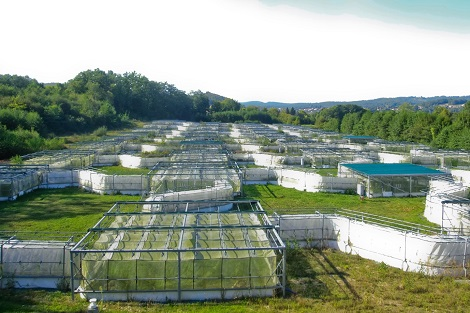
\includegraphics[width=6.cm]{metatron_0.jpg}
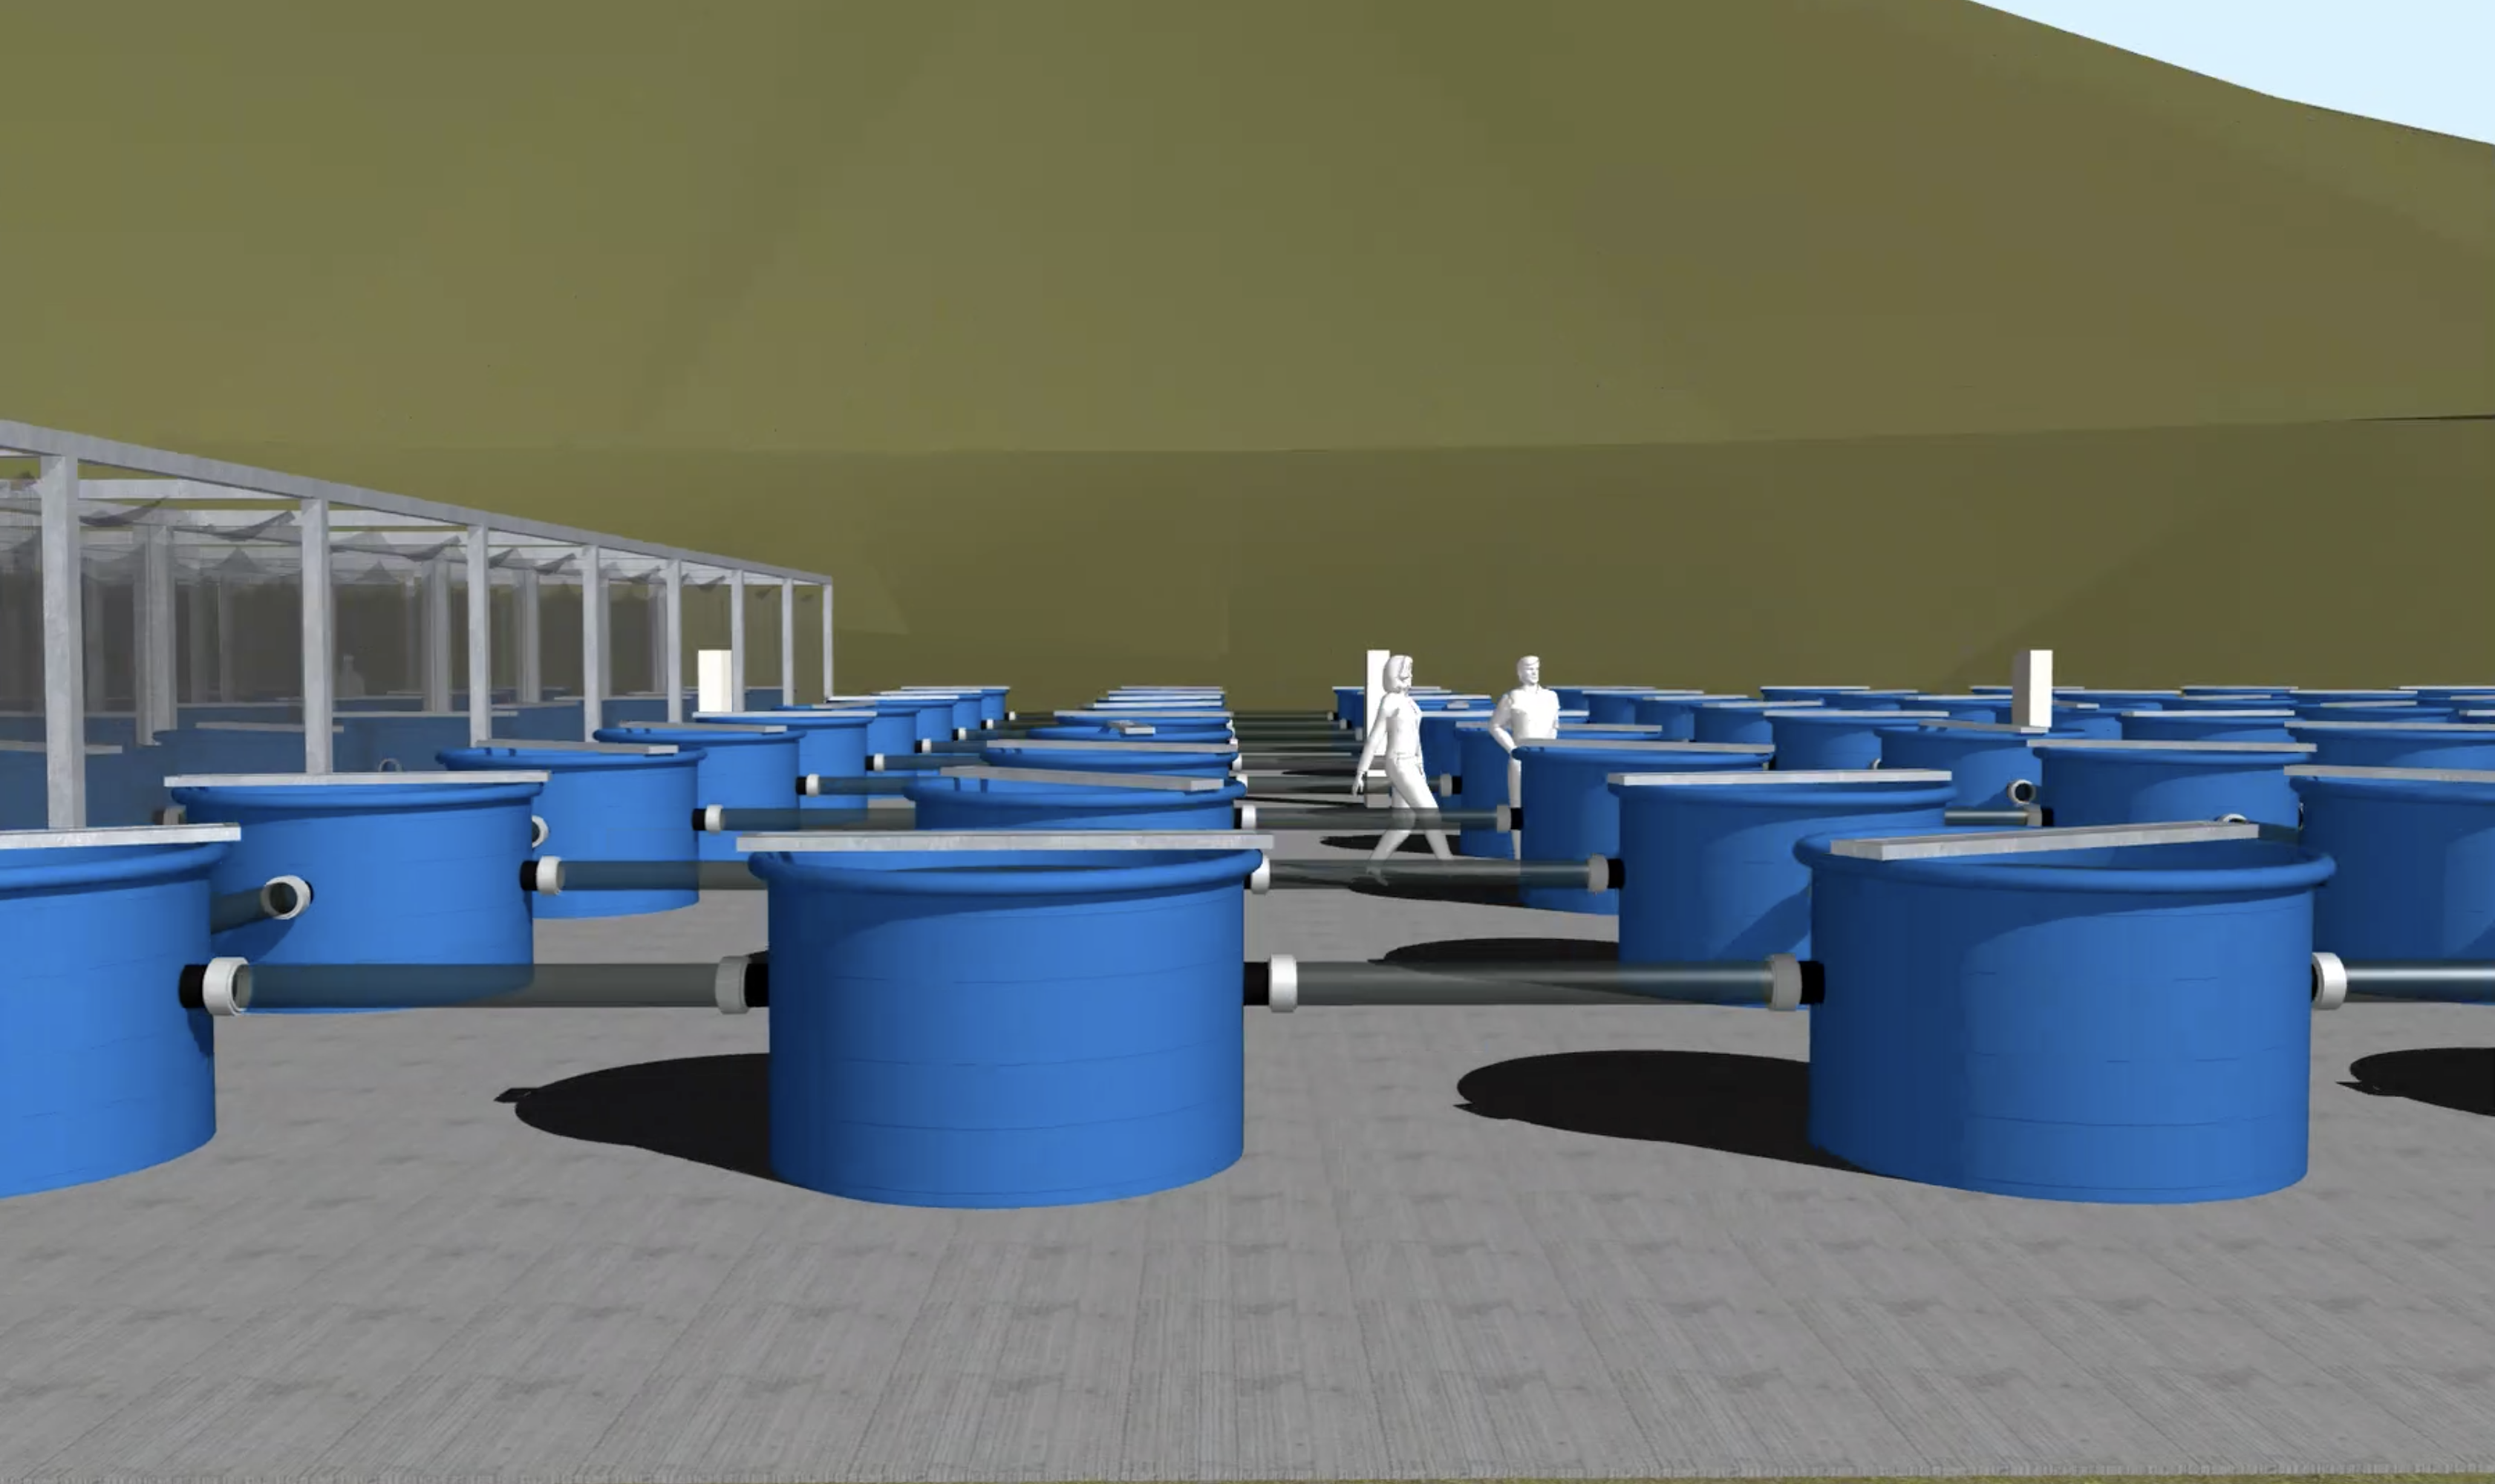
\includegraphics[width=6.cm]{aquatron.png}
\end{center}
\caption{\label{fig:temp}Left : Metatron, right : Aquatron}
\end{figure}

%% YZ: There's also the aqua-tron, that has recently been finished. You can talk to several people in Jose's team about it, if you're interested.


\paragraph{}
%Since 2012, the station hosts the Centre for Biodiversity Theory and Modelling (CBTM) \todo{now renamed Linking ...}
The centre for biodiversity theory and modelling (CBTM) \footnote{\url{http://www.cbtm-moulis.com}} 
%% YZ: Actually, not quite. The CBTM should still exist as a separate entity, in parallel to the "linking team". I think for your concerns, it might be simpler to just describe the CBTM...
aims to unify theories of biodiversity changes and of their consequences, in order to address the major challenges of the present biodiversity crisis.
%% YZ: I think you can say more than the previous sentence...
Lead by Jose M. Montoya\footnote{\url{http://www.cbtm-moulis.com/m-224-jose-m--montoya.html}}, the research ranges from phylogenetics to human interactions. Indeed, the ambition of the team is to give a theoretical framework to a general biodiversity science in order to deal with the present biodiversity crisis\footnote{\url{https://www.ipbes.net/news/Media-Release-Global-Assessment-Fr}}.

In practice, the team focus on several axes : generation of biodiversity and ecosystem services, the human nature interactions, habitat fragmentation and stability of ecological systems.

%% YZ: I guess you should state the axes right here. Otherwise, it is quite hard to follow.
The first axis focus on trying to understand how biodiversity change will affect ecosystem services. For example, how the loss of a species can affect crop production. However, because ecology and evolution theory are interrelated, the team integrates the role of eco-evolutionary dynamics in the responses of environmental changes. The same work is done for structure, dynamics and function of ecosystem, which are also interconnected \cite{bastazini_loss_2017} \cite{bideault_temperature_2019} \cite{galiana_geographical_2019}.



An additional axis is of human-nature interactions, which is studied in both directions : the human impact on biodiversity (habitat loss, fragmentation, global warming, etc.) which represent a threat of at least one in six species during this century, but also the feedback of biodiversity loss on human society. The aim is to study the long term sustainability of coupled social-ecological systems. Another objective is to better understand how biodiversity changes affect the services of the ecosystem, in particular  crop production and biological control in agricultural landscapes \cite{cazalis_we_2018} \cite{lafuite_sustainable_2018} \cite{montoya_trade-offs_2018} \cite{montoya_tradeoffs_2019}

% Habitat fragmentation and spatial dynamics of biodiversity
A particular case of human impact, landscape fragmentation which occurs at multiple spatial scales, is itself a subject of research: the habits loss itself as well as its effect ton he spatial dynamics of the ecosystem, with a special attention to metacommunities dynamics \cite{goncalves_habitat_2018} \cite{jacobi_operationalizing_2018}.

% Biodiversity and stability of ecological systems
Finally, a major focus of the team is studying the stability of ecological systems\footnote{\url{http://www.cbtm-moulis.com/m-214-biostases.html}}. Stability is an important feature of the ecosystem, and is a notion that is used in all previous research axes mentioned. The main research focus is to understand and quantify stability both in time and in space \cite{wang_stability_2017} \cite{zelnik_impact_2018}. However, since different stability measures are used in theory and experimental ecology, the team has tried to bridge the gap between these different measures and thus unify the notion of the stability \cite{arnold_examination_nodate}.
%% YZ: I am not sure barbier2019pyramids makes sense here. What measures is it bridging?
Different aspect of stability are studied: the link between the diversity of a species community and the stability of the community \cite{vallina2017phytoplankton}, the stability of meta-ecosystems \cite{arnoldi_particularity_2016} \cite{lurgi_effects_2016} \cite{wang_biodiversity_2016}.
Again, the sustainability of coupled social ecological systems are studied, in particular the role of human behavior in preventing the possible collapse of this systems.
%in as stability point of view (averting collapse for example).
%% YZ: This last sentence is quite strange.
Moreover, a mathematical framework is built by exploring the different notions of stability in order to link them \cite{arnoldi2016unifying} \cite{donohue_navigating_2016} and to know how to predict a critical changes by using experimental measures such as temporal variability \cite{arnoldi2016resilience} \cite{haegeman_resilience_2016} \cite{wang_invariability-area_2017}. 
% citation jusqu'a 2016 inclus



\newpage


\subsection*{Context}
\addcontentsline{toc}{subsection}{Context}







\subsection*{Ecosystem stability} % monitoring ?
\addcontentsline{toc}{subsection}{Ecosystem stability}

\paragraph{}
Ecosystems around the world are facing unprecedented disturbances due to increasing human intervention \cite{oosthoek_humanity_2005}. It is therefore important to analyse  their dynamics in the context of human perturbations, in order to both predicts the following state of the ecosystem and also to better manage it.
% complex dynamics
Nevertheless ecosystem dynamics can be notoriously complex, in particular due to the interactions between the different interconnected elements that constitute the system. %Thus, it is unavoidable to consider integrative study. 

\paragraph{}
\label{stability_litterature}
Ecologists are often interested in estimating stability far from equilibrium (as opposed to the classical physics approach, which focuses on studying stability near the equilibrium). Therefore, ecology needs to develop news tools to deal with understanding and predicting stability in complex dynamical systems. 
% resilience
One such concept, resilience, is traditionally used in theoretical studies, but is not the most relevant %\cite{arnoldi2016resilience}
\cite{gunderson_ecological_2000} \cite{neubert_alternatives_1997}.

Other stability measures are used to quantify the health of an ecosystem and follow its development over time, and are used to set accurate goals for the future planning management \cite {donohue_navigating_2016} \cite{mayer_strengths_2008}. A difficulty is that this word is used for many different meanings. One study has identified 163 definitions of 70 different stability concepts \cite{grimm_babel_1997}.

However, according to the same study, all these can be collapsed to only 6 pertinent concepts (constancy,  resilience,  persistence,  resistance,  elasticity and domain of attraction). Nonetheless, even if it is possible to reduce the number of the stability notions, several of them need to be used in order to consider the various aspects of stability, so as not to lose information on the behavior of the ecosystem \cite{derissen_relationship_2011}. There is thus a compromise between using too few measures, which will not capture all the relevant information, and using too many measures, which will not be practicable and may still not catch all the information \cite{hillebrand_decomposing_2018} \cite{donohue_dimensionality_2013}.
%Indeed, different stability measures have been defined to monitor different aspects of the system's response to perturbations. 
%If this different measures appear to be strongly related, it is not always true \cite{donohue2013dimensionality}.





%\paragraph{ecosystem management \\}
\paragraph{}

These different concept a main interest for ecosystem management \cite{mumby_ecological_2014}. It serves to anticipate the consequences of disturbances, in particular for anthropocentric ones. In the past decades, the field of ecosystem management has grown rapidly \cite{grumbine_reflections_1997} in response to the various modern disturbances, in order to sustain the integrity of ecosystem (including its structure, composition and function) \cite{jensen1994overview}. 

A major obstacle is to define measurable goal in order to have clear and trackable progress \cite{slocombe_forum:_1998}.
Even if it remains impossible to know all the exact processes operating within the ecosystem, it is still possible to understand the dominant behavior, which could be sufficient for ecosystem management \cite{mori_ecosystem_2011} \cite{slocombe_forum:_1998} \cite{stanley_ecosystem_1995}.
%\cite{mori2011ecosystem, slocombe1998defining, stanley1995ecosystem}







\subsection*{Forest fire}
\addcontentsline{toc}{subsection}{Forest fire}

\paragraph{}
As detailed previously, ecosystem  dynamics  can  be  notoriously  complex, in order to study the link between different notions of stability, a case studied is choose. 
We focus on forest fire management, as the dynamics of both forest and fire are well established. Nonetheless, the repercussions of fire management in forests, are not well understood, with much to be explored.


\paragraph{}
%\paragraph{forest disturbance \\}

Forest dynamics are affected by various disturbances. We define disturbance as events that can cause significant changes to the ecosystem \cite{white1985natural} \cite{rykiel_towards_1985} . Disturbance play an important role in forest ecosystem, notably by generating heterogeneity in the landscape \cite{turner2010disturbance}.

Disturbances can be defined by their duration \cite{perera_simulation_2015}. First, the disturbance who are considered instantaneous comparative to the dynamics of the forest (e.g. flood, windstorm, pest outbreaks ...).
Second, the constrain on long term, such as drought, temperature fluctuation or grazing.

Another useful distinction is the implication of human in the disturbance, even if it is not possible to isolate anthropogenic perturbations from natural ones \cite{perera_simulation_2015}.
Indeed, the human impact increases with time. For example, the area logged per year in Canadian forests has doubled between 1960 and 1995 \cite{smith_canadas_2000}. This logging disturbance could be relatively different from the natural ones.

%Also, some particular perturbations can be differentiate, the severe but rare events, this are termed "LIDS" for large and infrequent disturbances \cite{foster1998landscape}.
% rephrase if used this sentence. 

Finally, this different perturbations are often interrelated \cite{keane2015exploring}. This could create synergism between them \cite{mandre_environmental_2011} or have unanticipated responses \cite{perera_simulation_2015}. For example, fire and climatic fluctuations could interact to product cumulative effects \cite{romme_historical_2009}.



%\paragraph{Forest management \\}
\paragraph{}
For decades, sustainable forest management (SFM) has been used to maintain forest ecosystems \cite{macdicken_global_2015}. 
This practice serves to maintain different aspect of the ecosystem such as productive functions, biological diversity, and socioeconomic functions \cite{makela_using_2012}. 
However, its main target is to conserve the forest ecosystem as an unified entity. %\cite{franklin1989toward}.
%Moreover, there is no unanimity on this different facet of sustainability \cite{martinez-vega_assessing_2016}.
Also, the human demands from forests have broadened, making forest management more complex \cite{eggers_balancing_2017}. Several recent studies have shown that ecosystem management should try to reproduce the nature disturbance in order to preserve the dynamics of the forest \cite{bengston_changing_1994} \cite{bengtsson_biodiversity_2000}. 
According to \cite{hunter1990wildlife} and \cite{hunter1988paleoecology} it could be possible to imitate the size, frequency and severity of disturbances.

To reach this different target (mainly sustainability and productive functions), various criteria are used. To be practical, such criteria need follow some rules: be easily measured, be sensitive to stress, be anticipatory (to counter change), be integrative (consider different facets of forest ecosystem such soils, vegetation types ...) and have a low variability in response \cite{dale_challenges_2001}. However, monitoring programs typically consider only few indicators and fail to take into account the complexity of the ecosystem \cite{dale_challenges_2001}.


%\paragraph{Fire \\}
\paragraph{}

One on the main disturbances in forests is fire, and in some regions, it is the most significant one. Fires can create spatial patterns and heterogeneity in the landscape \cite{skinner_overview_nodate}. Fires also affect plant behavior, such that plants develop traits for adaptation to fire (thick  bark  and fire-stimulated flowering, sprouting, seed release and/or germination) \cite{mckelvey1996overview} \cite{chang1996ecosystem}.

Fires are also linked with other perturbations, mostly climatic variation \cite{mckenzie_climatic_2004}\cite{da2018dynamics}, by its effects to on fuel \cite{schoennagel_interaction_2004} and by weather \cite{fernandes_fire-smart_2013}. In practice, in some regions, fires are greatly affected by humans, wildfires have been considerably reduced due to the intervention of firefighters. Different management practices are used, depending notably on the country and the tree species, and mostly based on the misconception that lock the dynamics of a system will prevent it from collapse. That is why variability and collapse probability are the two measures choose in this study. In order to restore the natural dynamics of the forest, fires are sometimes allowed to run their course freely without intervention \cite{wallenius2011major}. 

Finally, one of the problem of the study of fire is its stochastic aspect and the variability in both space and time, which add complexity to the modelling of fire events and dynamics \cite{agee1998landscape} \cite{lertzman1998three}.

\newpage

\todo{expend (later)}

\subsection*{Synopsis}
\addcontentsline{toc}{subsection}{Synopsis}

\paragraph{}
The main purpose of the present document is to exhibit an ecosystem case where different notions of stability do not behave similarly. In order to do this, we look at how variability and collapse probability change with various model parameters, we consider different dynamical cases of the system, and describe the consequences for management practices.











%%%%%%%%%%%%%%%%%%%%%%%%%%%%%%%%%%%%%%%%%%%%%%%%%%%%%%%%%%%%%%%%%%%%%%%%%%%%%%%%%%%%%%%%%%%%%%%%%%%%%%%%
% Methods
%%%%%%%%%%%%%%%%%%%%%%%%%%%%%%%%%%%%%%%%%%%%%%%%%%%%%%%%%%%%%%%%%%%%%%%%%%%%%%%%%%%%%%%%%%%%%%%%%%%%%%%%

\newpage
\section{Methods}


\subsection{Model}


\paragraph{}
We consider a model of a forest fire, with $N$ being live biomass and $W$ dead wood. The living biomass is defined like standing alive tree and dead wood is dead wood debris and standing dead trees \cite{russell2015quantifying}.

The living biomass follow a logistic growth \cite{tsoularis2002analysis} \cite{jensen1975comparison} with an allee effect \cite{stephens1999allee} \cite{amarasekare1998allee}. On the other hand, the evolution of the dead wood is proportional to the density of $N$ and decay with time \cite{kahl_wood_2017} \cite{shorohova_stump_2012} \cite{christensen_estimation_1977} \cite{delaney_quantity_1998} \cite{barbosa_decomposition_2017} \cite{fravolini_quantifying_2018} \cite{wilson_dynamics_2005} \cite{zielonka_dynamics_nodate}.

Both $N$ and $W$ are affected by fire, with a stronger effect for $W$ (the dead wood burn easier than $N$). A fire occur when $t\in F$ the set of fire events. The severity of the fire is assumed to follow an exponential law of average $strength$. Finally, the severity of the fire is proportional the density biomass $N$ and $W$ with a greater importance for $W$ \cite{martinson_fuel_2013} \cite{safford_effects_2009} \cite{lecomte_effects_2006}.

\paragraph{}

\[
\left\lbrace
\begin{array}{rcl}
\frac{dN}{dt} & = & gN(1-N/K)(N/a-1) - \delta_F(t)s(t)(N+\alpha W) \\
\\
\frac{dW}{dt} & = & mN -dW - \beta\delta_F(t)s(t)(N+\alpha W) \\
\end{array}
\right.
\]

The major assumption of the model is that fire frequency is independent of fuel density, it will be argued later that do not question the following results of this study.

Another assumption is that fire need fuel ($W$) to burn. In other words, when $W=0$, fire stop. It is based on the fact that fire are manly driven by fuel \cite{schoennagel_interaction_2004} \cite{stephens_effects_2012} \cite{syphard_comparing_2011} \cite{safford_effects_2009} \cite{stephens_experimental_2005}.

Also, we consider only density biomass and do evaluate the spatial distribution of both density and fire severity \cite{bergeron_natural_2002}.

Same, we consider only one type of forest. Indeed, it have been argued that different type of forest fire could be differentiate (crown fires, light surface fires ... ) \cite{heinselman_1981_fire}.
% fire severity proportional to the density of $N$ and $\alpha W$


\paragraph{}\todo{useful to give value ? (and justify with paper) it is not that simple, it could be a mess ... }\todo{all value at least positive non null, and m lower than max(dn / dt)}

This model used $9$ parameters, 5 for growth therms and 4 for the fire model.

The first one $g$ is the grow rate of the living biomass. $K$ is the forest's carrying capacity. 

The allee effect threshold $A$ represent the minimum quantity of living biomass in order to survive. In other words, if the dynamics of $N$ go below $A$, the system collapse. The possible value of $A$ are between $0$ and $1$, but in practice $A$ take low value, typically between $0.02$ and $0.2$.

For the growth part of dead wood, $m$ is the decay rate of living biomass (the rate of conversion from $N$ to $W$) and $d$ the decay rate of $W$ itself.

Now, for the fire term, $\beta$ is the coefficient that represent the fact that $W$ burn easier than $N$. $\delta_F(t)$ and $s(t)$ represent respectively the fire occurrence and the severity of an eventual fire at the time $t$. \todo{beta and alpha bigger than $1$}

Finally, similar to $\beta$, $\alpha$ represent the fact that $W$ burn easier than $N$.





\paragraph{}
In order to simplify the study of the model, we adimensionnalise the system. We have anymore only 7 parameter (\hyperref[adim]{calculus in appendix}). The adimensionnalise system is the following :

\[ % adim model
\left\lbrace
\begin{array}{rcl}
\frac{dN}{dt} & = & N(1-N)(N-A) - \delta_F(t)s(t)(N+\alpha W) \\
\\
\frac{dW}{dt} & = & mN -dW - \beta\delta_F(t)s(t)(N+\alpha W) \\
\end{array}
\right.
\]

\paragraph{estimation of "reasonable" coefficient for this model%, sometimes easier to find "reasonable" coefficient, $K$ not anymore present, but not always ...
} \todo{}


%\paragraph{Remark} % equilibrium
\paragraph{} % equilibrium
To help understand the dynamics of the model used, we give some simple analytic result. to do this, we only consider growth terms.

\[ % adim model
\left\lbrace
\begin{array}{rcl}
\frac{dN}{dt} & = & N(1-N)(N-A) \\
\\
\frac{dW}{dt} & = & mN -dW \\
\end{array}
\right.
\]

\paragraph{}
We have thus 3 equilibrium, 2 stable $(0, 0)$ and $(1, \frac{m}{d})$ and one unstable $(A, \frac{mA}{d})$ (\hyperref[equi]{calculus in appendix}).

\paragraph{}
Also, the figure below give an example for a well choose set of parameters of a time series. We can see that here the dynamics come back to the stable equilibrium $(1, \frac{m}{d})$ most of the time, except for the last fire when the system collapse to go to the other stable equilibrium $(0, 0)$. \todo{strength the temporal series (final time = 300)}

\begin{figure}[h!]
\centering
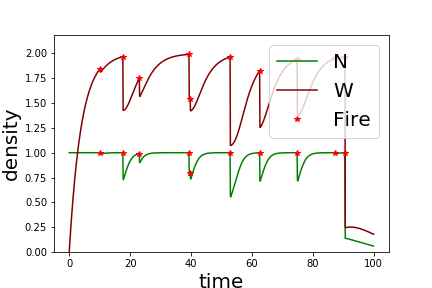
\includegraphics[width=6cm]{return_between_2.png}
\caption{Time series example}
%\label{fig:universe}
\end{figure}

\newpage
\paragraph{}
Also we represent the phase portrait for both $N$ and $W$. We recall that the dynamics of $W$ depend of the value $N$. 
%%%%% same parameters set for both

\begin{figure}[h!]
\centering
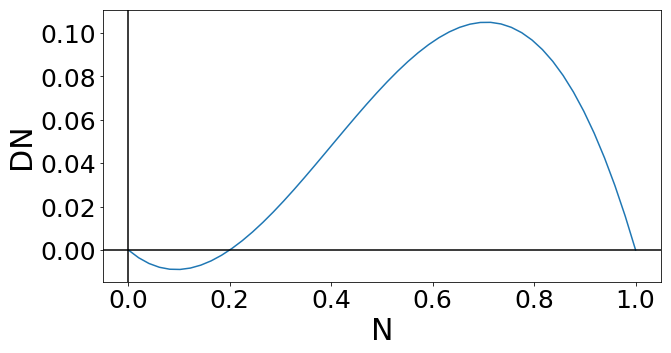
\includegraphics[width=6cm]{phase_N.png}
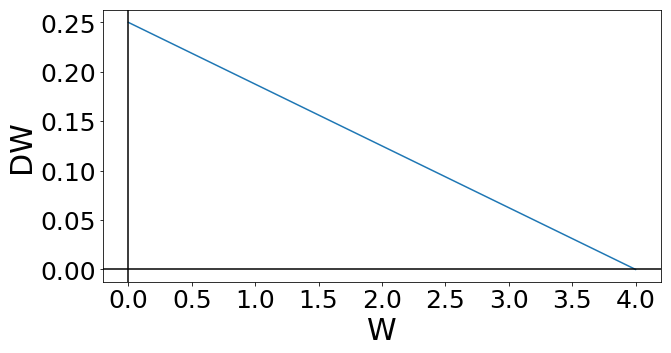
\includegraphics[width=6cm]{phase_W.png}
\caption{Phase portrait}
%\label{fig:universe}
\end{figure}

\paragraph{}
We can remark that the growth of the system is continuous and deterministic. However, the perturbation (fire) are discrete and stochastic. The implementation to solve the sytem need thus to take care of this, more details in \hyperref[technicality]{appendix}.
%\todo{I have already 2-3 papers about this, re found, cite}




\paragraph{}
\label{average_estimation}
Also, in order to not have to run too long simulation, an average of both $N$ and $W$ is estimated. It help to initialise the dynamics, indeed the transitions time is shorter

An analytic expression is given, mainly based on the assumptions that frequency is high enough to consider that the global dynamics of the system is continuous (\hyperref[average]{calculus in appendix}).


\[
\left\lbrace
\begin{array}{rcl}
N^{av} & = & \frac{1+a+\sqrt{(1-a)^2-4\gamma}}{2} \\
W^* & = & \epsilon N^* \\
\end{array}
\right.
\]

With,
\[
\left\lbrace
\begin{array}{rcl}
\epsilon & = & \frac{m-\beta s f}{d + \beta s f \alpha} \\
\gamma & = & sf(1+\alpha\epsilon)
\end{array}
\right.
\]

\paragraph{}
We can check below that average are well estimated, even for low value of frequency.

\begin{figure}[h!]
\centering
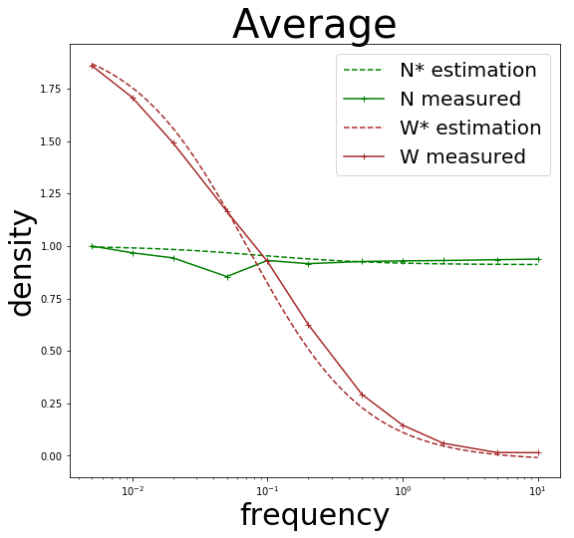
\includegraphics[width=9cm]{average.png}
\caption{Average $N^{av}$ and $W^{av}$}
%\label{fig:universe}
\end{figure}




%%%%%%%%%%%%%%%%%%%%%%%%%%%%%%%%%%%%%%%%%%%%%%%%%%%%%%%%%%%%%%%%%%%%%%%%%%%%%%%%%%%%%%%%%%
%%%%%%%%%%%%%%%%%%%%%%%%%%%%%%%%%%%%%%%% Measures %%%%%%%%%%%%%%%%%%%%%%%%%%%%%%%%%%%%%%%%
%%%%%%%%%%%%%%%%%%%%%%%%%%%%%%%%%%%%%%%%%%%%%%%%%%%%%%%%%%%%%%%%%%%%%%%%%%%%%%%%%%%%%%%%%%

\newpage
\subsection{Measures}

\paragraph{}
One of the main interest of forest management is to avoid collapse. That is why we study the collapse probability of the system. In the present model, a collapse is report when the density value of living biomass go below the allee thresholds, indeed, when it happens, the dynamics of both $N$ and $W$ converge to $0$.

\todo{example when after the collapse, it remains $N$ and $W$, which keep decreasing, and strength the time series (ft = 300)} % here we can think it will always going to 0 because only of the fire.


\newpage

\begin{figure}[h!]
\centering
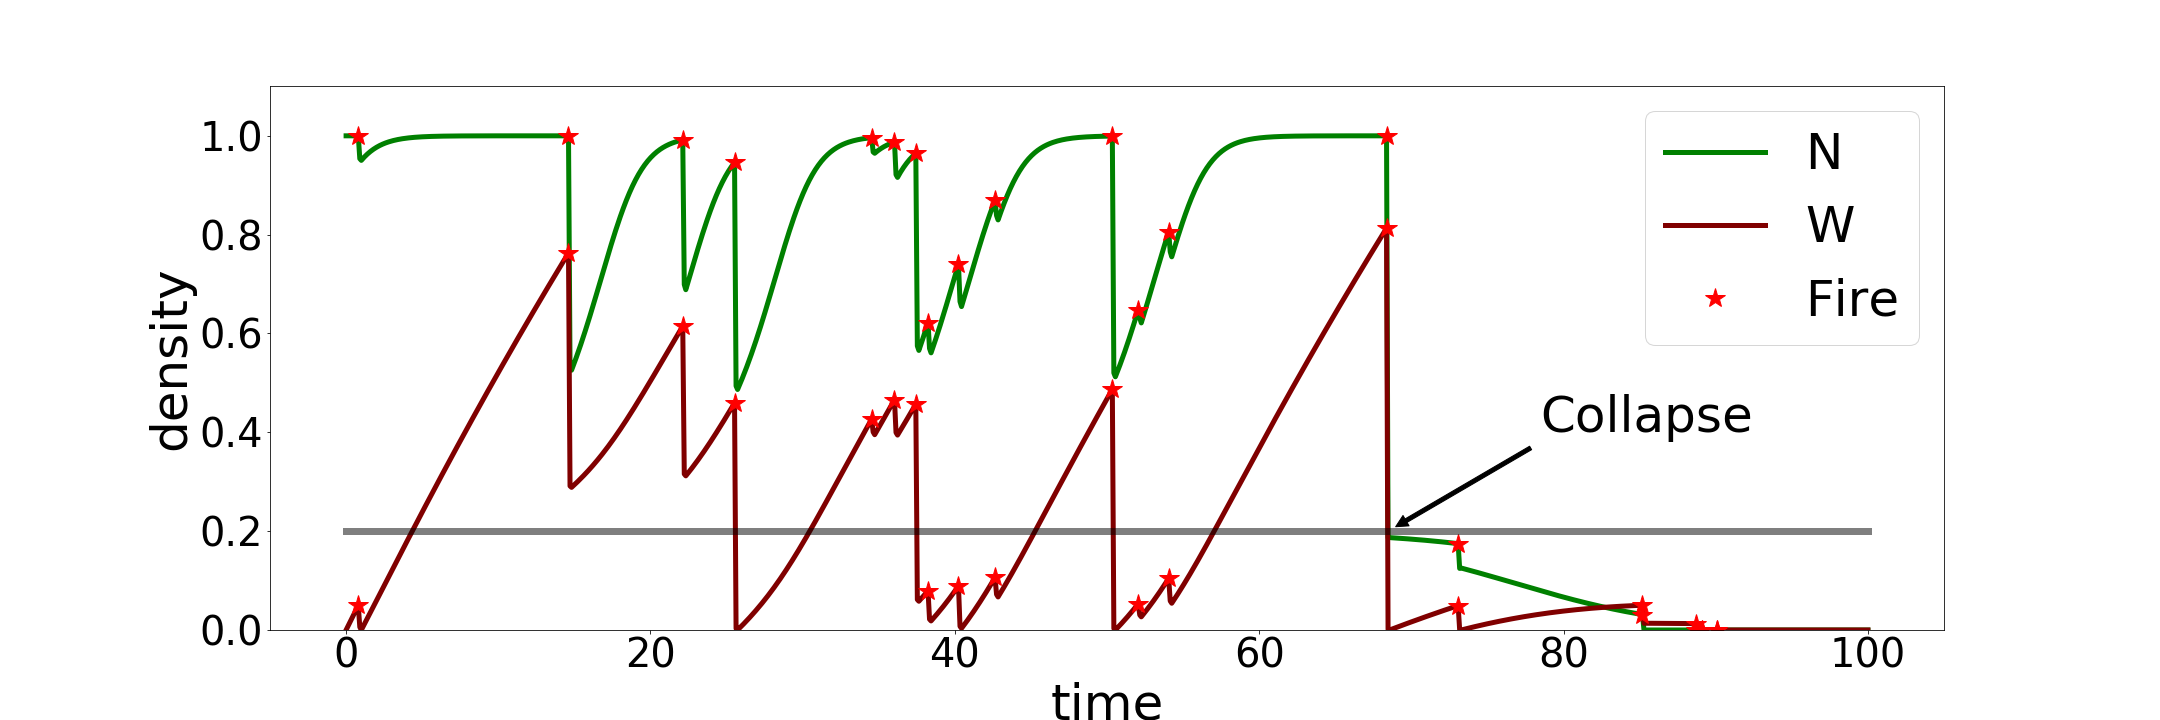
\includegraphics[width=10.cm]{time_series_cp_1.png}
\caption{Average : $N^{av}$ and $W^{av}$}
%\label{fig:universe}
\end{figure}


\paragraph{}
Measuring collapse probability need to run several simulation to approximate it. However, it will depend on the time study used. Indeed, more the time study is long, the more is the risk to collapse. Even if it could be enough to used always the same time study, we present an improvement of this measure : probability to collapse by time unit. This upgrade is thus independent of the time study choose (details in \hyperref[proba_per_time_unit]{appendix}).


\paragraph{} % why variability ?
\todo{why variability ?}
\begin{itemize}
    \item lock dynamics (\todo{I have 2 papers})
    \item because it could give an indication of collapse 
    \begin{itemize}
        \item tests of the predicted effect of population variability (PV) have yielded variable, controversial results. Several studies provide apparent support for the predicted positive relationship (Karr 1982;Pimm et al. 1988; Forney \& Gilpin 1989; Bengtsson \& Milbrink 1995). Other studies reveal no significant relationship (Bengtsson 1989; Pollard \& Yates 1992) or provide evidence for a negative relationship (Schoener 1991; Schoener \& Spiller 1992; Lima et al. 1996; for discussions of the statistical validity of several of these studies see Diamond \& Pimm 1993; Pimm 1993; Tracy \& George1993; Gaston \& McArdle 1994).
        
        numerous theoretical treatments besides those described above (MacArthur \& Wilson 1967; MacArthur 1972; Richter-Dyn \& Goel 1972; Leigh 1975, 1981; Belovsky 1987; Goodman 1987) yield the same prediction: increased population variability leads to increased extinction risk.
        
        \todo{Some authors (MacArthur 1972; Diamond 1984; Pimm et al. 1988) have argued that the rate  of extinction should be directly related to population variability. Al- though intuitively appealing, this relationship may not hold, especially when population density and absolute population variability are positively correlated (Tracy and George 1992; Schoener and Spiller 1992) \cite{rutledge1976ecological}}
        \todo{ (N),Population size of mature individuals (and trend in population size, were clearly the best predictors of extinction risk) \cite{ogrady_what_2004}}
    \end{itemize}
\end{itemize}


\paragraph{}
Variability is defined like the variance when a collapse has not occur yet. Indeed, a collapse of the system will induce a bias in the computation of variability.


\begin{figure}[h!]
\centering
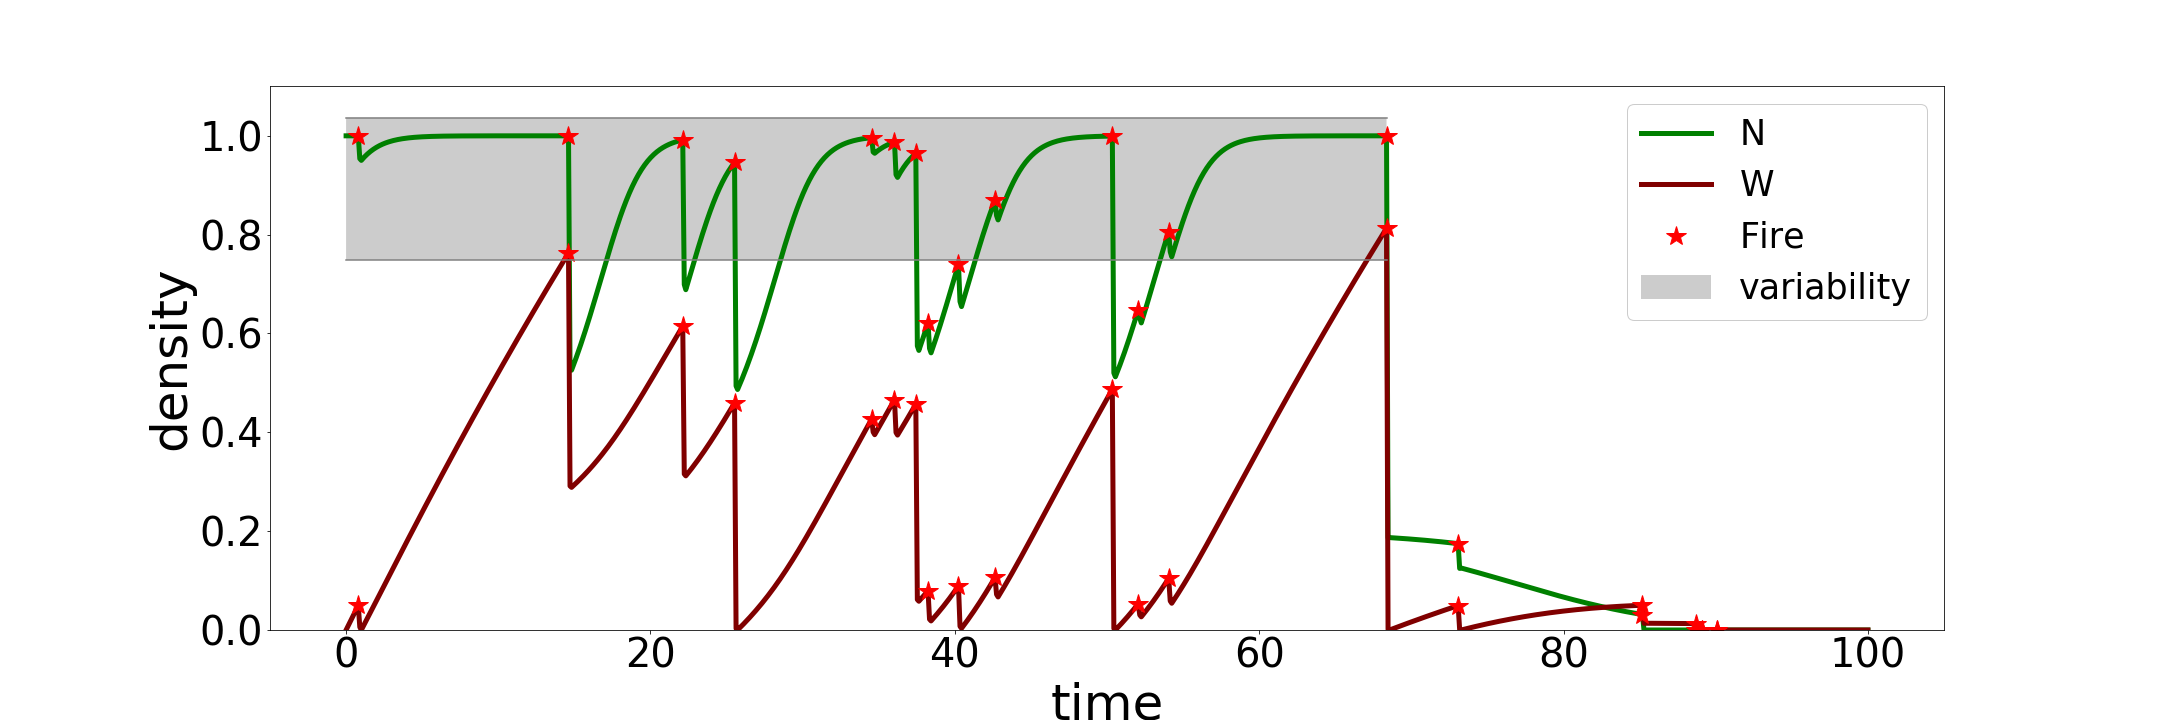
\includegraphics[width=10.cm]{time_series_sd_1.png}
\caption{Average : $N^{av}$ and $W^{av}$}
%\label{fig:universe}
\end{figure}



\paragraph{}
In practice, we have to make compromise to decrease different bias. Even if the dynamics is initialise close to the average approximation, it is safer to not take into account the first time of the time series to compute collapse probability (thus we do not consider the first $10\%$ of the time series). Also, as explain previously, it make no sens to compute variability after a collapse occurs, but in order to use the same time to measure variability, we restrict at the second $10\%$ of the time series. Indeed, the bias of time series not used because they collapse to soon is here quite low (\hyperref[algo_variability]{algorithm in appendix}). Other way to measure variability have been implemented and could be found in \hyperref[other_variability]{appendix}.

\todo{same plot as previously but with variability between $10\%$ and $20\%$}


\paragraph{}
A similar measure to variability is the coefficient of variability. Defined as the variability over the mean. Indeed, a good measure of variability will be independent of the mean abundance if the dynamics are the same, but will not be independent if the dynamics change with mean abundance \cite{gaston_measurement_1993}\cite{noauthor_temporal_1994}


\paragraph{}
The main problem is : bias when collapse \todo{Variability analysis should be performed on data that are free from artefact \cite{seely2004complex} }, thus (to decoupled this two phenomenon) : 
\begin{itemize}
    \item use the same simulation
    \item same fire \todo{More time means more variation \cite{lawton1988more} }
    \item same time
    \item \paragraph{}
        Instead of doing a lot of simulation and average the effect, used only one simulation (only one fire). One problem is that when we change the frequency, we need to choose between used the same time scale, and so not take the same fire (it will truncated) or used the same fire and so no have the same time scale. Because both are relevant, both are computed. 
        
        We can remark that "same fire" tend to be more robust in the sens that it is more smooth.
\end{itemize}


\paragraph{} % estiamtion
Numerical approximation of measures have two main drawback. Firstly, lot of time is needed, especially if we want to have a robust approximation (and so used long time simulation) and / or if we want to compute measure on a lot of parameters sets. Also, numerical approximation of measures do not give direct information of which and how parameters affect the measures. 
Thus, both collapse probability and variability are analytically estimated.

\paragraph{} % estimation variability
The estimation of variability is based on the assumption that the two density $N$ and $W$ remain close to their \hyperref[average_estimation]{average estimated} by $N^{av}$ and $W^{av}$. 

We denote $\lambda$ the average severity of a fire, estimated by
\[
\lambda = min(\{s(N^*+\alpha W^*), \frac{W^*}{\beta s (N^*+\alpha W^*)}\})
\]
We make the assumption that the effect of fire are independent (which is true when the dynamics is close to linear).
And so, we predict the variability with, \cite{zelnik_impact_2018}
\[
variability = f\frac{\lambda^2}{U}
\]
Details in \hyperref[variability_estimation]{appendix}

\todo{figure for just this estimation of variability}
\begin{figure}[h!]
\centering
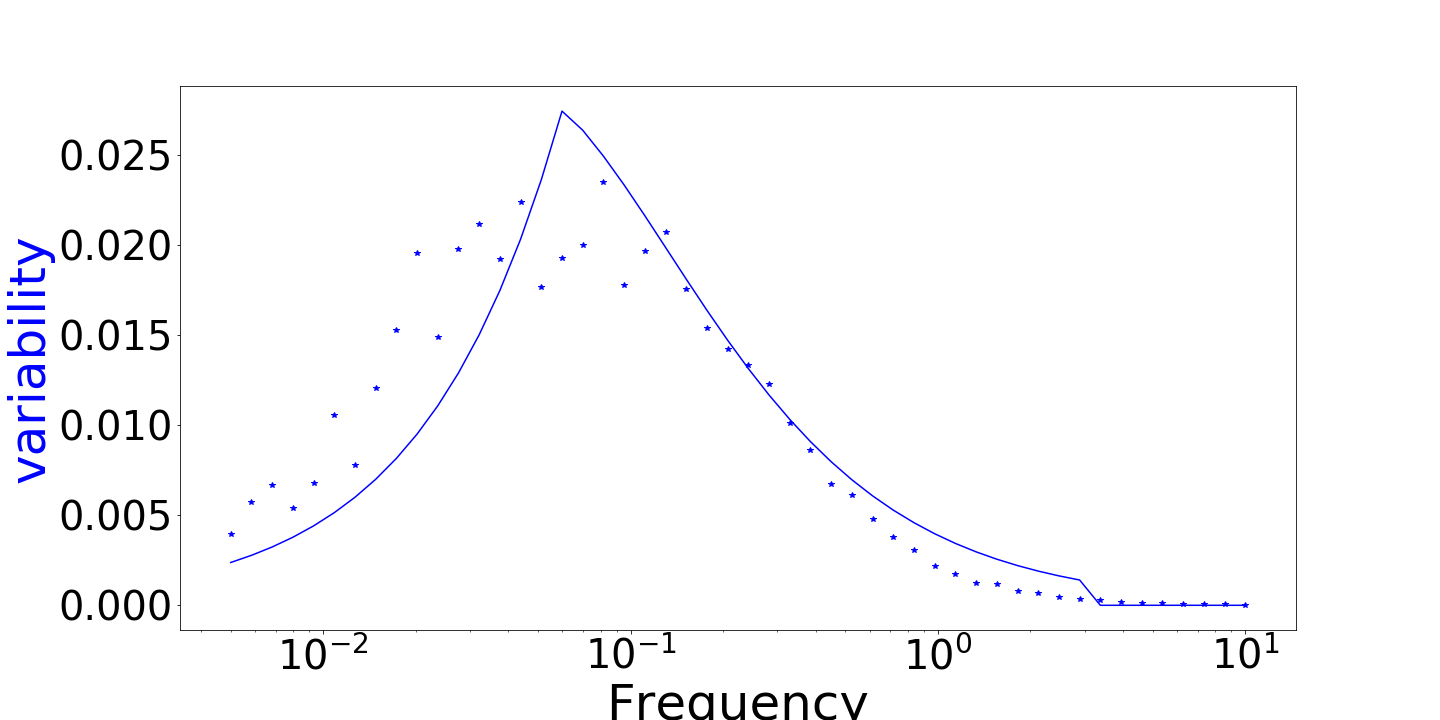
\includegraphics[width=10.cm]{variability_good.png}
\caption{Variability estimation}
%\label{fig:universe}
\end{figure}

\paragraph{}
Of course, the precision of this estimation depend greatly to the parameters region. For example, on the figure below, we can see that the approximation is less accurate. We can see ... \todo{depend on the plot ... describe what is the difference}

Generally, when the total severity of the fire is high, the accuracy of the estimation decreases. In practice, the product of the parameter $s.\alpha.\beta$ give an interesting clue of the precision of the variability estimation.

Other estimation of variability have been implement and are presented in \hyperref[variability_estimation_other]{annexes}.

\todo{make agian the plot with just the used estimation (just the "good" ones)}
\begin{figure}[h!]
\centering
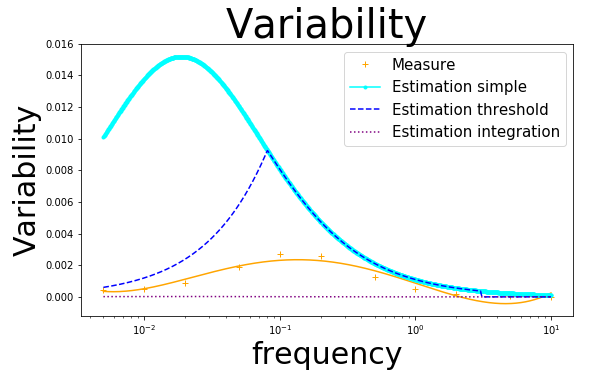
\includegraphics[width=10.cm]{variability_2.png}
\caption{Variability estimation}
%\label{fig:universe}
\end{figure}


\paragraph{}
Same as variability, we also estimate the collapse probability.

For this, we assume that the system can only collapse with a unique fire. This probability is called $cp1$. Derivation could be found \hyperref[cp_derivation]{appendix}
\[
\begin{array}{rcl}
cp1 & = & (N^*+\alpha W^*)((N^*-a+s)\exp(-\frac{N^*-a}{s}) - (\frac{W^*}{\beta}+s)\exp(-\frac{W^*}{s\beta})
\end{array}
\]
This probability is considered to follow a binomial law.
\[
\begin{array}{rcl}
cp & = & 1-(1-cp1)^{fT} \\
\end{array}
\]

\paragraph{}
Here again, the estimation work generally quite well, but the correctness dependent greatly on the set of parameter.

More generally, even if the maximum of the collapse probability is under estimated, the location of the peak is quite well predicted. As previously, the biases increase with the severity of the fire.


\todo{do again the plot with a the left work well, and not very well for the right.}
\begin{figure}[h!]
\centering
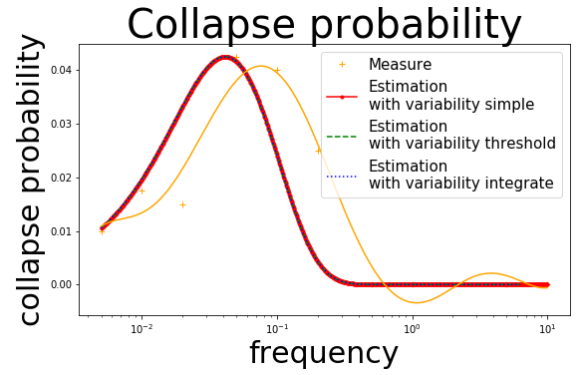
\includegraphics[width=6.cm]{cp.png}
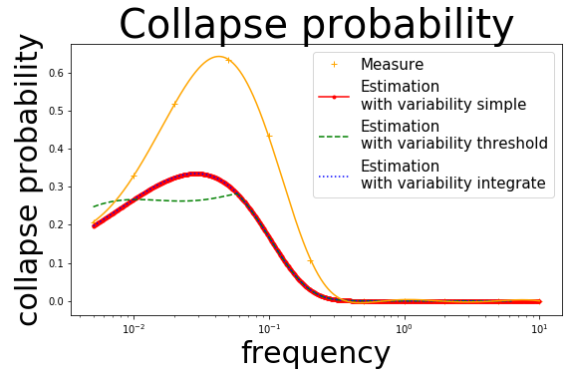
\includegraphics[width=6.cm]{cp_threshold.png}
\caption{Cp estimation}
%\label{fig:universe}
\end{figure}



\paragraph{}
In this study, we focus on two measures : variability and collapse probability. However as details in the introduction, several different notion of \hyperref[stability_litterature]{stability} are established. This different aspect of stability are briefly presented in  \hyperref[stability_others]{appendix}.


\subsection{Dynamics cases}

\paragraph{}
In order to better understand the dynamics of the system, we distinguish different cases (and later subcases). Indeed, this facilitate the study, because we can so study case by case the different dynamics and their respective consequences.

\paragraph{}
Because we want to explore exhaustively the different dynamics cases, we introduce a coefficient to distinguish typical cases. Different \hyperref[other_ratio]{others coefficients} have been tested but only the following is used. After, another axes will be used to subdivide each cases.

For the first axis, we introduce the ratio called "r" which is an approximation of the average of density burned over the average of growth. This is useful to discern the predominance between the growth of W and the density burned of W. For example, if $r$ is low, growth predominates the fire effect.
\[
r = fs\beta(\frac{2}{m}+\frac{\alpha}{d})
\]
A more details derivation of this ratio is given is \hyperref[derivation_ratio]{appendix}.


\paragraph{}
We can so distinguish a gradient of two extreme case with an intermediate one. The first one, when "$r$" is low, is called "return to equilibrium". The dynamics is quite simple : most of the time $W$ have the time to come back near $W^{eq}$ before another fire occur.
\begin{figure}[h!]
\centering
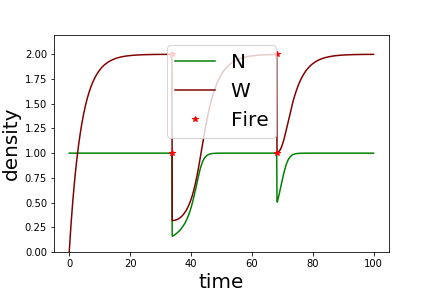
\includegraphics[width=3.9cm]{return_to_eq_1.png}
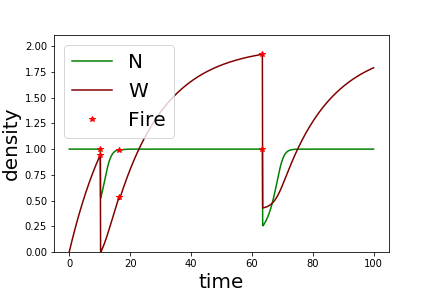
\includegraphics[width=3.9cm]{return_to_eq_2.png}
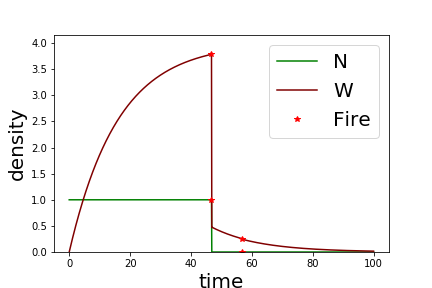
\includegraphics[width=3.9cm]{return_to_eq_3.png}
\caption{Return to equilibrium}
%\label{fig:universe}
\end{figure}



\paragraph{}
At the opposite, when the ratio called $r$ is high, in another word when fire tend to annihilate the growth of $W$, this one remains low. 
\begin{figure}[h!]
\centering
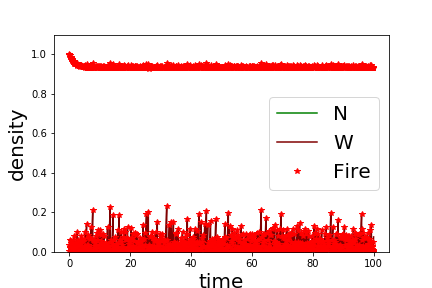
\includegraphics[width=3.9cm]{continue_1.png}
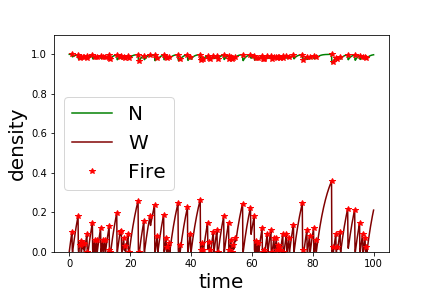
\includegraphics[width=3.9cm]{continue_2.png}
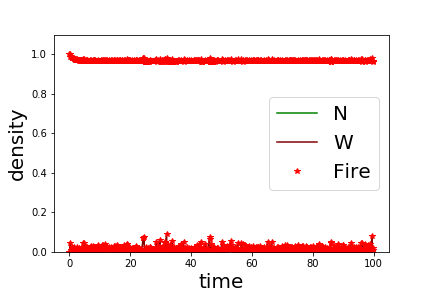
\includegraphics[width=3.9cm]{continue_3.png}
\caption{Fuel low}
%\label{fig:universe}
\end{figure}


\paragraph{}
Between the two previous cases, we define a third cases called "equivalent". It happens when the effect of the fire and the growth are about the same quantity. In this case, $W$ can take the larger range of value (from $0$ to $W^{eq}$).
\begin{figure}[h!]
\centering
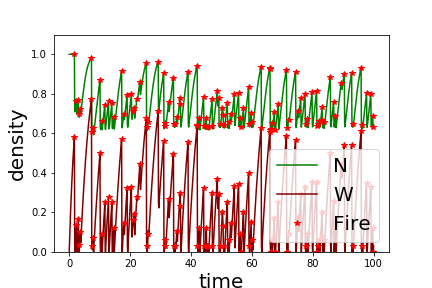
\includegraphics[width=3.9cm]{middle_1.png}
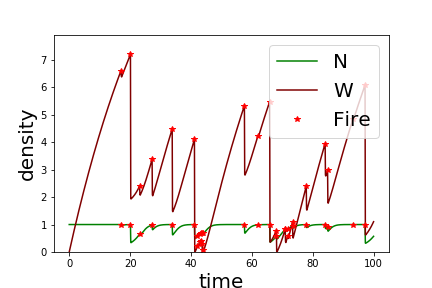
\includegraphics[width=3.9cm]{middle_2.png}
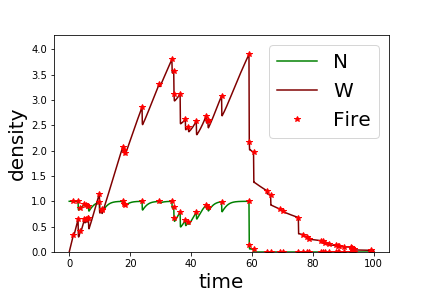
\includegraphics[width=3.9cm]{middle_3.png}
\caption{Equivalent}
%\label{fig:universe}
\end{figure}


\paragraph{}
Also, in order to visualise the limit of each cases, examples for each limits are presented

\begin{figure}[h!]
\centering
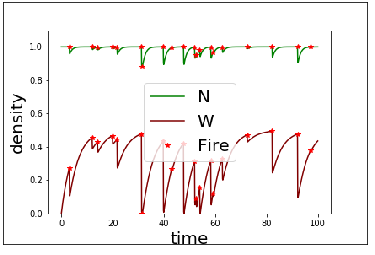
\includegraphics[width=3.9cm]{lim_eq_middle_1.png}
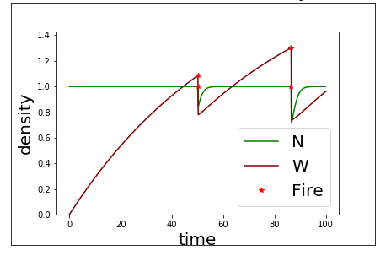
\includegraphics[width=3.9cm]{lim_eq_middle_2.png}
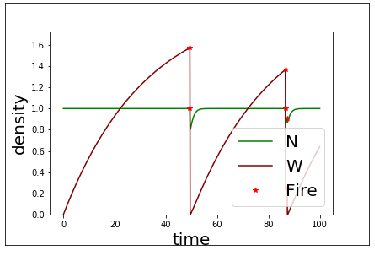
\includegraphics[width=3.9cm]{lim_eq_middle_3.png}
\caption{Limit return to equilibrium / equivalent}
%\label{fig:universe}
\end{figure}


\begin{figure}[h!]
\centering
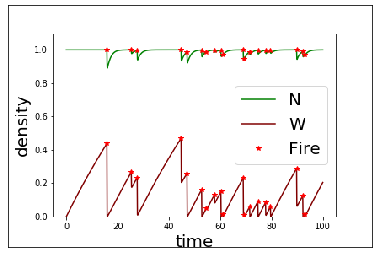
\includegraphics[width=3.9cm]{lim_c_middle_1.png}
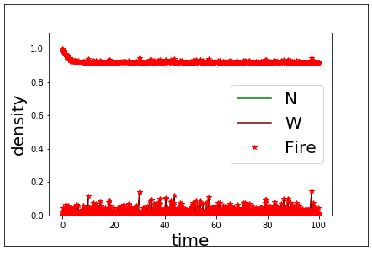
\includegraphics[width=3.9cm]{lim_c_middle_2.png}
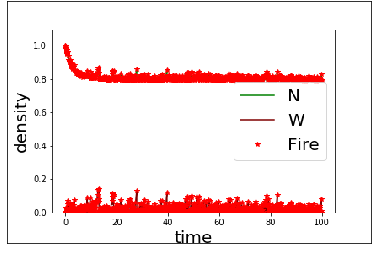
\includegraphics[width=3.9cm]{lim_c_middle_3.png}
\caption{Limit fuel low / equivalent}
%\label{fig:universe}
\end{figure}



%%%%%%%%%%%%%%%%%%%%%%%%%%%%%%%%%%%%% subcases %%%%%%%%%%%%%%%%%%%%%%%%%%%%%%%%%%%%%%%%%%%%%%%%%%

\newpage


\subsubsection{"Return to equilibrium"}

\paragraph{}
Now, we study the case called "return to equilibrium more deeply. For this, we divided again the case in three sub-cases. To discriminate this three cases, we mainly consider the risk to collapse. Effectively, here, the dynamics return to the equilibrium after most of the fire, thus, we can easier study when a collapse is possible and when is inevitable.

\paragraph{} % never
Firstly, for same set of parameter, it is impossible to collapse. This could occur for two different meaning. The first one is when they are never enough fuel to maintain a fire strong enough to collapse the forest.
Because we consider to be at the equilibirum,
\[
\left\lbrace
\begin{array}{rcl}
     N & = & 1 \\
     W & = & \frac{m}{d} \\
\end{array}
\right.
\]
Thus, the quantity burned in only one fire can not be higher than $\frac{m}{d}$. \\
Formally,
\[
\begin{array}{rcl}
s\beta(N+\alpha W) & = & s\beta(1+\alpha \frac{m}{d}) \\
& < & W \\
& < & \frac{m}{d} \\
\end{array}
\]
Also, for the first equation (for $N$) we have a collapse only if
\[
\begin{array}{rccl}
                &  s(N+\alpha W) & > & N-a \\
\Leftrightarrow &  s(1+\alpha \frac{m}{s}) & > & 1-a \\ 
\Leftrightarrow &  \frac{m}{d\beta} & > & 1-a \\ 
\Leftrightarrow &  \frac{m}{d( 1-a)} & > & \beta \\ 
\end{array}
\]
Thus, if this condition is not respected (in practice when $\beta$ is high enough) it is impossible to have a collapse. When can see below  an example when the lack of $W$ prevent the collapse of the forest.

\begin{figure}[h!]
\centering
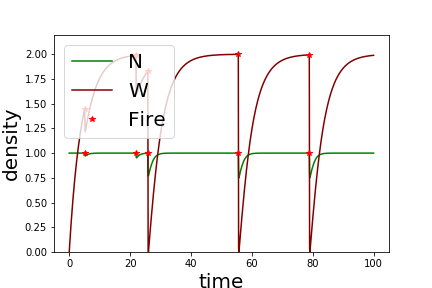
\includegraphics[width=9cm]{return_never_1.png}
\caption{Never collapse}
%\label{fig:universe}
\end{figure}

\newpage
\paragraph{}
Also, it is unlikely (no more certainty) to collapse if the severity of the fire is really low (compare to $N = 1$). We say that the system is unlikely to collapse if the probability to collapse with only one fire is lower than $0.01$.
\[
\begin{array}{rccl}
                &  P(s(N+\alpha W) > N-a ) & < & 0.01 \\
\Leftrightarrow &  P(s(1+\alpha \frac{m}{d}) > 1-a ) & < & 0.01 \\ 
\Leftrightarrow &  P(s > \frac{1-a}{(1+\alpha \frac{m}{d})} ) & < & 0.01 \\ 
\Leftrightarrow &  \exp(-\frac{1-a}{s(1+\alpha\frac{m}{d})}) & < & 0.01 \\ 
\end{array}
\]


\begin{figure}[h!]
\centering
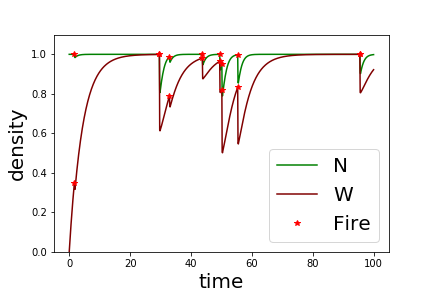
\includegraphics[width=9cm]{return_never_2.png}
\caption{Never collapse}
%\label{fig:universe}
\end{figure}


\paragraph{} % always
At the opposite, for some set of parameter, the system always collapse. Of course, it occurs, when the condition $\frac{m}{d( 1-a)} > \beta$ is respected. Also, the severity of the fire need to be strong enough to collapse. Same as previously,
\[
\begin{array}{rccl}
                & P(s(N+\alpha W) > N-a ) & < & 0.01 \\
\Leftrightarrow & \exp(-\frac{1-a}{s(1+\alpha\frac{m}{d})}) & > & 0.2 \\ 
\end{array}
\]


\begin{figure}[h!]
\centering
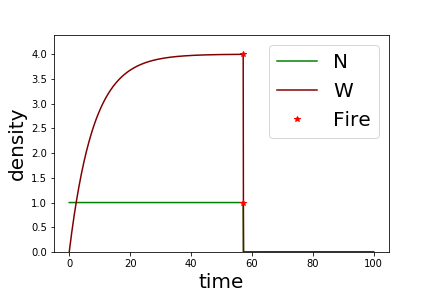
\includegraphics[width=3.9cm]{return_always_1.png}
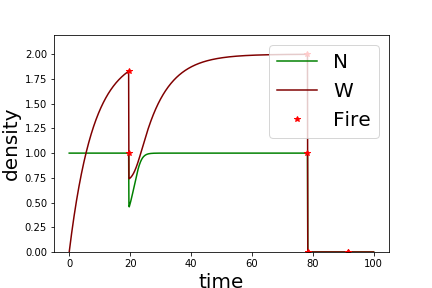
\includegraphics[width=3.9cm]{return_always_2.png}
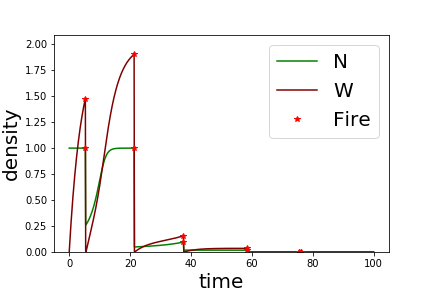
\includegraphics[width=3.9cm]{return_always_3.png}
\caption{Always collapse}
%\label{fig:universe}
\end{figure}




%\todo{préciser que le temps d'étude n'est pas tjrs suffisant pour le constater}
\paragraph{} % between
Between this two extremes sub-cases, exists a range of parameters when a collapse could occur. This happen, when $W$ is high enough and also when the actual strength of the fire is high enough;


\begin{figure}[h!]
\centering
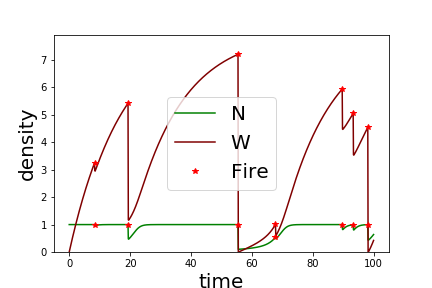
\includegraphics[width=3.9cm]{return_between_1.png}
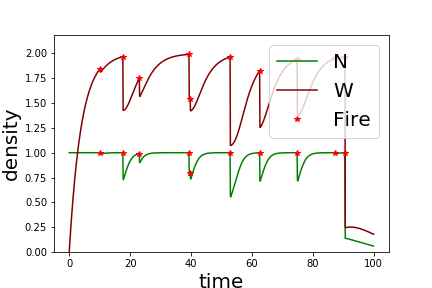
\includegraphics[width=3.9cm]{return_between_2.png}
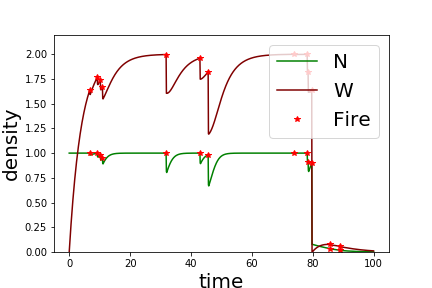
\includegraphics[width=3.9cm]{return_between_3.png}
\caption{Intermediate case}
%\label{fig:universe}
\end{figure}



%%%%%%%%%%%%%%%%%%%%%%%%%%%%%%%%%%%%%%%%%%%%%%%%%%%%%%%%%%%%%%%%%%%%%%%%%%%%%%%%%%%%%%%%%%%%%%%%
%%%%%%%%%%%%%%%%%%  \todo{... link with cp (but after) ... } %%%%%%%%%%%%%%%%%%%%%%%%%%%%%%%%%%%
%%%%%%%%%%%%%%%%%%%%%%%%%%%%%%%%%%%%%%%%%%%%%%%%%%%%%%%%%%%%%%%%%%%%%%%%%%%%%%%%%%%%%%%%%%%%%%%%

\subsubsection{"Fuel low"}

\paragraph{}
Following the same idea than previously, when $W$ is always low, collapse can never occurs. In practice, we can observe a collapse only, when the set of parameter is closed to the case "intermediate". So, $W$ can go higher enough to generate a fire. But this is observed rarely. On the figure below we can observe that $W$ come back to $0$ with each fire and have no time to accumulate to engender a strong fire.
%\todo{jamais collapse, expliquer pourquoi avec un très simple calcul}
%\todo{nuancer dans le cas ou on est proche du cas "equivalence" and fuel is not always low enough}


\begin{figure}[h!]
\centering
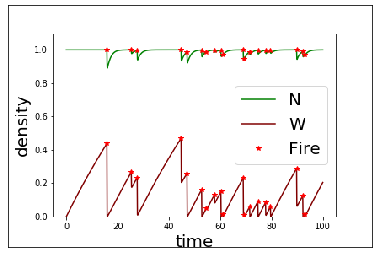
\includegraphics[width=12cm]{lim_c_middle_1.png}
\caption{Fuel low}
%\label{fig:universe}
\end{figure}


\newpage
\subsubsection{"Equivalent"}
%\todo{extrapoler, on divise en 2 cas pour s'approcher des 2 autres cas}
%\todo{quand proche continuous, collapse happen if fuel go too high}
%\todo{illustrate}

\paragraph{}
The case called "equivalent" is the harder to study. Thus, we extrapolate the previous results to this case. To do this, we divided arbitrarily the case in two. We use the ratio "$r$" for this. When "$r$" is higher we assume we are relatively close to the case "fuel low". Here, we can collapse when the fuel grow fast enough (relatively to the fire frequency) to accumulate enough fuel and be able to collapse.

\begin{figure}[h!]
\centering
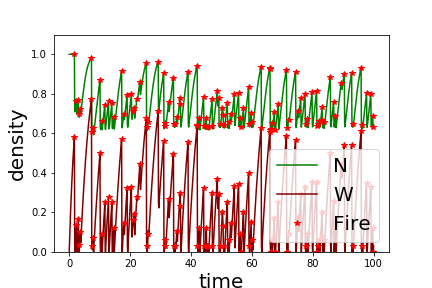
\includegraphics[width=3.9cm]{equivalent_high_1.png}
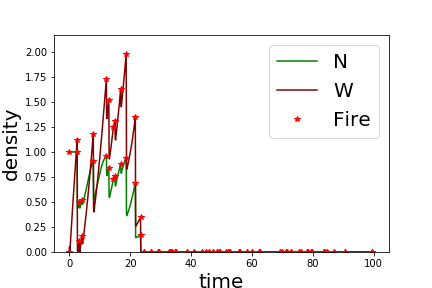
\includegraphics[width=3.9cm]{equivalent_high_2.png}
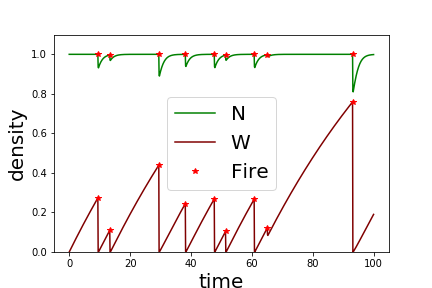
\includegraphics[width=3.9cm]{equivalent_high_3.png}
\caption{Case : Equivalent, but close to "fuel low"}
%\label{fig:universe}
\end{figure}

\paragraph{}
Also, when "$r$" is lower, we use again the three sub-cases (from the case "return to equilibrium") to characterise the dynamics of the system. We can observe that for this example, the dynamics do not change much, and that the extrapolation could make sense (but only if $r$ is low enough).
%\todo{ratio low, proche "return", on herite des 3 cas, never always, between}
%\todo{illustrer 3 exemples pour chaque cas}

%\paragraph{}

\begin{figure}[h!]
\centering
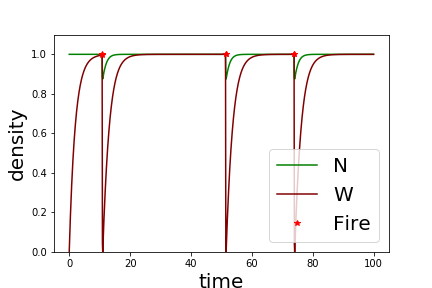
\includegraphics[width=3.9cm]{equivalent_low_never_1.png}
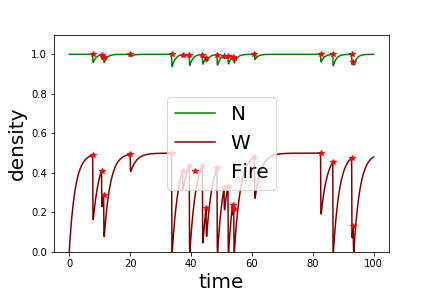
\includegraphics[width=3.9cm]{equivalent_low_never_2.png}
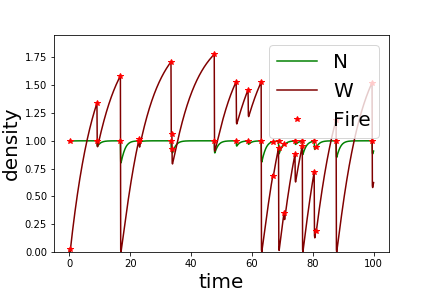
\includegraphics[width=3.9cm]{equivalent_low_never_3.png}
\caption{Case : Equivalent, never collapse}
%\label{fig:universe}
\end{figure}


%\paragraph{}

\begin{figure}[h!]
\centering
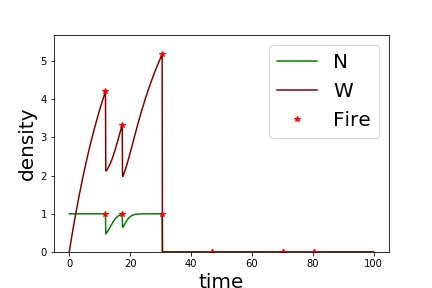
\includegraphics[width=3.9cm]{equivalent_low_always_1.png}
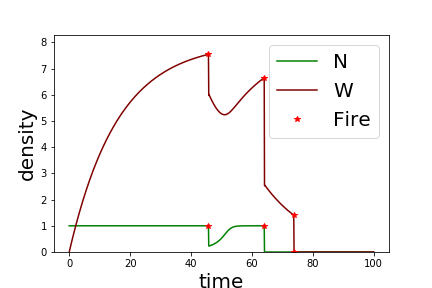
\includegraphics[width=3.9cm]{equivalent_low_always_2.png}
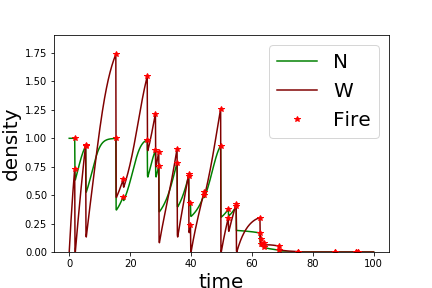
\includegraphics[width=3.9cm]{equivalent_low_always_3.png}
\caption{Case : Equivalent, always collapse}
%\label{fig:universe}
\end{figure}



%\paragraph{}

\begin{figure}[h!]
\centering
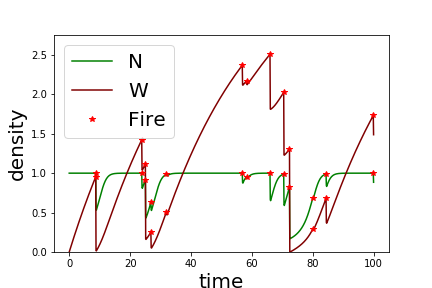
\includegraphics[width=6cm]{equivalent_low_between_1.png}
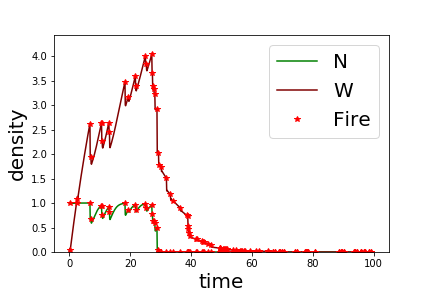
\includegraphics[width=6cm]{equivalent_low_between_2.png}
\caption{Case : Equivalent, intermediate case}
%\label{fig:universe}
\end{figure}



\todo{link dynamics cases with scenarios management (explain that they are a link "between dynamics" cases and "scenarios management" however it is two different concept)}

\todo{consequences for cp and variability}

%%%%%%%%%%%%%%%%%%%%%%%%%%%%%%%%%%%%%%%%%%%%%%%%%%%%%%%%%%%%%%%%%%%%%%%%%%%%%%%%%%%%%%%%%%%%%%%%%%%%%%%%%%%%%%%%%%
% Result
%%%%%%%%%%%%%%%%%%%%%%%%%%%%%%%%%%%%%%%%%%%%%%%%%%%%%%%%%%%%%%%%%%%%%%%%%%%%%%%%%%%%%%%%%%%%%%%%%%%%%%%%%%%%%%%%%%


\newpage
\section{Results}

%\subsection{Link literature model}

%\begin{itemize}
%    \item link collapse probability and the parameter (enough data ?)
%    \item link variability with the parameter in the literature ? ? ? 
%\end{itemize}


\subsection{Link between variability and cp}

\begin{itemize}
    \item explain the idea of the loop (we have already talk in the methodology about the link between varaibility and cp ... )
    \item show the loop in different case \todo[color=purple]{demonstrate that we have found all the possible cases (use case dynamics and/or estimation)}
    \item illustrate different part of the loop with numerical simulation to give an intuition (show time series for the following cases)
    \begin{itemize}
        \item no cp no var
        \item high variability low cp
        \item high variability high cp
    \end{itemize}

    \item link with dynamical cases (for each sub cases plot a representative plot)
    \itme use estimation (exploit them numerically) to "understand the "shape" of the loop. (illustrate when we are in typical case, for example return to equilibrium, AND when we change from one case to another one)
    \item use numerical simulations to study the location of the peak (study the order and the distance (on frequency scale) between the different peaks (variability, collapse probability and average) )
    \item (same fire, same time ...) in order to better understand how the variability changed (it is a method ... ) demonstrate numerically that they are still a peak of variability (we can now know that it is not an artefact of cp)
\end{itemize}

\subsection{Implication for management}


\paragraph{}
fuel removal, very efficient to decrease cp

\paragraph{}
In drought perturbation, we have a decrease of variability but an increase to the collapse probability \todo[color=purple]{EXTEND THIS RESULT, check, illustrate}







%%%%%%%%%%%%%%%%%%%%%%%%%%%%%%%%%%%%%%%%%%%%%%%%%%%%%%%%%%%%%%%%%%%%%%%%%%%%%%%%%%%%%%%%%%%%%%%%%%%%%%%%%%%%%%%%%%
% Discussion
%%%%%%%%%%%%%%%%%%%%%%%%%%%%%%%%%%%%%%%%%%%%%%%%%%%%%%%%%%%%%%%%%%%%%%%%%%%%%%%%%%%%%%%%%%%%%%%%%%%%%%%%%%%%%%%%%%
\newpage
\section{Discussion}
\todo{Try to not make repetition (or not too much)}







\subsection{Model}


\paragraph{}
We assume that the frequency of the fire is independent of the density biomass. It can be argued that fuels have an influence on both severity and frequency  of fires \cite{schoennagel_interaction_2004}. However, adding this feedback (from $W$ to the frequency) will surely tends to decrease the density biomass of $W$ (because, when $W$ is higher, the frequency is higher too, and so the dynamics keep a low value of $W$). In other word, this should to have the "management fuel" scenarios more often

Also, we only consider one kind of death wood, this can be details in several type (coarse woody debris, fine woody debris, below ground ...) \cite{russell_quantifying_2015}. In the literature, the data are rarely for all the wood, and, some wood burned easier than other. 

Moreover, in practice we can distinguish several fire regime (e.g., crown fires, severe surface fires, and light surface fires) \cite{reichle_fire_1981}. All of this different fires disturbed differently the dry wood. So the dynamic can be modelled in a more complex ways.

Less relevant, we only consider density biomass. However, the spatial distribution can affect fires propagation (especially for small fires). For example, a burned area can create an obstacle when another fire occur \cite{bergeron_natural_2002}.

Even if fire is the main perturbation of the system, other disturbances can be relevant, like mechanical thinning \cite{liu_analyzing_2010}\cite{schoennagel_interaction_2004}\cite{wimberly_assessing_2009}.


\subsection{Link literature model}

\paragraph{}
Data varies greatly and also depend on several variable (type of forest, localisation ... )


\subsection{Technicality about variability}

\paragraph{}
Because the collapse of the system affect the variability of this system, it is difficult to have robust computation of the variability. None of the different variant of the variability presented above are perfect which is biased. "Variability all" compute the variance even if the system collapse, which tend to decrease a lot the variability. 
    
Also, "variability only" who compute the variability only when the system do not collapse, is biased because the variability could be not be the same when the system will collapse or not. (We do not catch the link between variability and the collapse off the system). And if the system always collapse (which can be the case, especially for long time study) we do not have an estimation of the variability. 

On the other hand, "variability until" used all the simulation, but the time of the study is never the same.

More generally, because collapse can occur at different time (or never) it is difficult to have a robust computation of the variability.



\subsection{Technicality about collapse probability}

\begin{itemize}
    \item collapse probability depend of the time of the study
    \item problem when cp is too high, to have enough data on the variability
    \item also, problem to have a measure who depend on a numerical parameter
    \item solution : used collapse probability per time units
\end{itemize}



\todo[color=purple]{collapse indicators ?}

\newpage
%%%%%%%%%%%%%%%%%%%%%%%%%%%%%%%%%%%%%%%%%%%%%%%%%%%%%%%%%%%%%%%%%%%%%%%%%%%%%%%%%%%%%%%%%%%%%%%%%%%%%%%%%%%%%%%%%%
% Conclusion
%%%%%%%%%%%%%%%%%%%%%%%%%%%%%%%%%%%%%%%%%%%%%%%%%%%%%%%%%%%%%%%%%%%%%%%%%%%%%%%%%%%%%%%%%%%%%%%%%%%%%%%%%%%%%%%%%%

\section*{Conclusion}
\addcontentsline{toc}{section}{Conclusion}


\subsection*{Synthesis}
\addcontentsline{toc}{subsection}{Synthesis}


\subsection*{Opening}
\addcontentsline{toc}{subsection}{Opening}

\paragraph{}
Talk about a more general / different problem ...


\newpage

\section*{personal review}
\addcontentsline{toc}{section}{Personal review}


\newpage
\addcontentsline{toc}{section}{Bibliography}
%\bibliographystyle{plain}
%\bibliographystyle{alpha}
%\bibliographystyle{apalike}
\bibliographystyle{plainnat}

%\bibliography{references}
\bibliography{references_zotero,references}




\newpage
\appendix
\addcontentsline{toc}{section}{Annexes}

\newpage
\section{Adimensionnalisation}
\label{adim}

\todo{calculus to Adimensionnalise the system}


\newpage
\section{Equilibrium}
\label{equi}
\todo{write the calculus of equilibrium and stability}



\newpage
\section{Technicality}

\label{technicality}
\subsection{Solve the system}

\paragraph{}
problem : compute a continuous dynamics with discrete disturbances \\
solution : use classical solver between each fire and stop the solver when a fire occur to compute and remove the biomass


\subsection{Choice of the time step}
illustrate the problem of the choice of the time step, according to the frequency.

\subsection{}
Time of the study



\newpage
\section{Average estimation}
\label{average}

\paragraph{}
in order to not have to run too long simulation, an average of both $N$ and $W$ is estimated. It help to initialise the dynamics, indeed the transitions time is shorter
\todo{ ? ? ? (plot time series in appendices, to compare if we take the initial point [1.,0] or $[1,\frac{m}{d}]$ explain that in this case we need to have really long simulation especially if $d$ the recovery rate is too small)}

We use the following model :
\[
\left\lbrace
\begin{array}{rcl}
\frac{dN}{dt} & = & N(1-N)(N-A) - \delta_F(t)s(t)(N+\alpha W) \\
\frac{dW}{dt} & = & mN -dW - \beta\delta_F(t)s(t)(N+\alpha W) \\
\end{array}
\right.
\]
Assumption : frequency is high enough : 
\[
\begin{array}{rcl}
\delta_F(t) & \approx & f \\
s(t) & \approx & s \\
\end{array}
\]
With $f$ the average frequency of the fire and $s$ the average strength of the fire.


\[
\left\lbrace
\begin{array}{rcl}
\frac{dN}{dt} & = & N(1-N)(N-A) - f s (N+\alpha W) \\
\frac{dW}{dt} & = & mN -dW - \beta f s (N+\alpha W) \\
\end{array}
\right.
\]
At the pseudo equilibrium (when fire counterbalance growth).
\[
\left\lbrace
\begin{array}{rcl}
\frac{dN^*}{dt} & = & 0 \\
\frac{dW^*}{dt} & = & 0 \\
\end{array}
\right.
\]
Focus on the second equation : 
\[
\begin{array}{rcl}
\frac{dW^*}{dt} & = & 0 \\
mN^*-dW^* -\beta f s (N^*+\alpha W^*) & = & 0 \\
(m-\beta s f)N^* - (d+\beta f s \alpha) W^* & = & 0 \\
W^* & = & \frac{m-\beta s f}{d + \beta s f \alpha} N^*
\end{array}
\]
Notation
\[
\begin{array}{rcl}
\epsilon & = & \frac{m-\beta s f}{d + \beta s f \alpha} \\
\end{array}
\]
Thus
\[
W^* = \epsilon N^*
\]
For the first equation
\[
\begin{array}{rcl}
N^*(1-N^*)(N^*-A) - f s (N^*+\alpha W^*) & = & 0 \\
-AN^*+(1+A)N^{*^2}-N^{*^3} -f s (1+\alpha\epsilon)N^* & = & 0 \\
-(A+f s (1+\alpha\epsilon))N^*+(1+A)N^{*^2}-N^{*^3} & = & 0 \\
\end{array}
\]
Denote $\gamma = sf(1+\alpha\epsilon)$. 
\begin{equation}
-(A+\gamma)N^*+(1+A)N^{*^2}-N^{*^3} = 0
\end{equation}
The trivial solution $N^* = 0$ have no interest (in this case, both alive and death biomass are $0$).
\[
\begin{array}{rcl}
-(A+\gamma)+(1+A)N^{*}-N^{*^2} & = & 0 \\
\end{array}
\]

\[
\begin{array}{rcl}
\Delta & = & (1+A)^2 - 4(A+\gamma) \\
& = & (1-A)^2 - 4\gamma \\
\end{array}
\]
For now, we assume it is positive. %\todo{use it to delimit cases ?}
In practice, it is enough to have the product $f.s$ low enough %(here $f$ is high, but it is still possible to decrease $s$.
\[
\left\lbrace
\begin{array}{rcl}
N_1^* & = & \frac{1+a-\sqrt{(1-a)^2-4\gamma}}{2} \\
N_2^* & = & \frac{1+a+\sqrt{(1-a)^2-4\gamma}}{2}
\end{array}
\right.
\]
By using (1), because $\gamma$ and $A$ are both positives, we can deduce from the order of the solution $(0, N_1^*, N_2^*)$ that $N_1^*$ is unstable and $N_2^*$ is stable. 
\\
We are only interested in the stable solution, so, from now, we use the notation $N^* = N_2^*$.



\begin{figure}[h!]
\centering
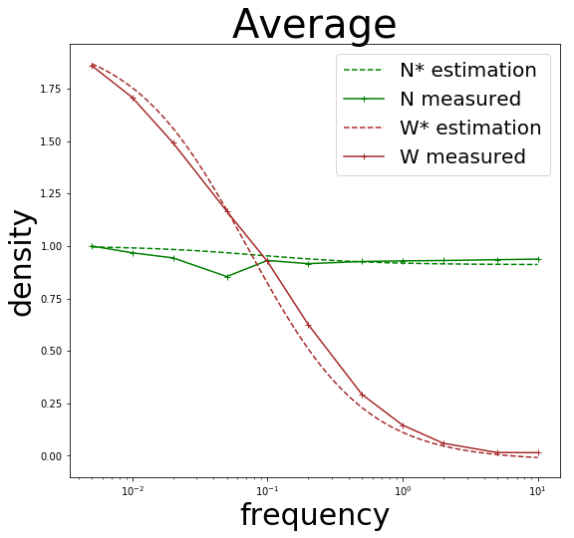
\includegraphics[width=7cm]{average.png}
\caption{Estimation and measures of the average of $N$ and $W$}
%\label{fig:universe}
\end{figure}

\paragraph{Remark}
Sometimes, the approximation of $W^*$ take negative value. Because $W$ can not be negative, we only consider the positive part of $W^*$.




\newpage
\section{proba per time unit}
\label{proba_per_time_unit}

\todo{exact derivation}
\todo{algorithm}
\todo{plot to check / illustrate}


\newpage
\section{Variability}

\subsection{algo variability}
\label{algo_variability}
\todo{algo variability}

\subsection{other variability}
\label{other_variability}
\todo{other variability, present them, their advantages, drawback, and their algorithm}


\newpage
\section{variability estimation}
\subsection{variability estimation derivation}
\label{variability_estimation}
\todo{variability estimation}

\subsection{variability estimation other}
\label{variability_estimation_other}
\todo{variability estimation other}



\newpage
\section{cp derivation}
\label{cp_derivation}
\todo{}

\newpage
\section{Stability}
\subsection{stability others}
\label{stability_others}
\todo{talk about others "measures of stability" such as skewness, kurtosis ... }


\subsection{General notions of stability}
\todo{Talk about the general concept of stability (across the different disciplines)}


\newpage
\section{others coefficients}
\label{other_ratio}



\newpage
\section{derivation ratio}
\label{derivation_ratio}

\todo{rewrite, it is not clear for now}

\end{document}
